\documentclass[12pt,a4paper,oneside]{book}

% ============================================================
% PACKAGES
% ============================================================
\usepackage[utf8]{inputenc}
\usepackage[T1]{fontenc}
\usepackage[french]{babel}
\usepackage{graphicx}
\usepackage{geometry}
\geometry{top=2.5cm, bottom=2.5cm, left=3cm, right=2.5cm}
\usepackage{setspace}
\onehalfspacing
\usepackage[hidelinks]{hyperref}
\usepackage{listings}
\usepackage{xcolor}
\usepackage{fancyhdr}
\usepackage{tocbibind}
\usepackage{float}
\usepackage{titlesec}
\usepackage{lmodern}
\usepackage{enumitem}
\usepackage{caption}
\usepackage{subcaption}
\usepackage{tabularx}
\usepackage{booktabs}
\usepackage{multicol}
\usepackage{tikz}
\usetikzlibrary{shapes.geometric, arrows, positioning, fit}

% ============================================================
% COULEURS & STYLES
% ============================================================
\definecolor{inptblue}{RGB}{0, 51, 102}
\definecolor{inptred}{RGB}{204, 0, 0}
\definecolor{codegreen}{rgb}{0,0.6,0}
\definecolor{codegray}{rgb}{0.5,0.5,0.5}
\definecolor{codepurple}{rgb}{0.58,0,0.82}
\definecolor{backcolour}{rgb}{0.97,0.97,0.95}

\lstdefinestyle{mystyle}{
    backgroundcolor=\color{backcolour},
    commentstyle=\color{codegreen},
    keywordstyle=\color{blue},
    numberstyle=\tiny\color{codegray},
    stringstyle=\color{codepurple},
    basicstyle=\ttfamily\scriptsize,
    breakatwhitespace=false,
    breaklines=true,
    captionpos=b,
    keepspaces=true,
    numbers=left,
    numbersep=5pt,
    showspaces=false,
    showstringspaces=false,
    showtabs=false,
    tabsize=2,
    frame=single,
    rulecolor=\color{codegray}
}
\lstset{style=mystyle}

% En-tete / Pied de page
\pagestyle{fancy}
\fancyhf{}
\fancyhead[L]{\small\nouppercase{\leftmark}}
\fancyhead[R]{\small Cloud Priv\'e OpenStack}
\fancyfoot[C]{\thepage}
\renewcommand{\headrulewidth}{0.4pt}
\renewcommand{\footrulewidth}{0.2pt}

% ============================================================
% PAGE DE GARDE PROFESSIONNELLE
% ============================================================
\begin{document}

\begin{titlepage}
\begin{tikzpicture}[remember picture, overlay]
  % Bande bleue en haut
  \fill[inptblue] (current page.north west) rectangle ([yshift=-4cm]current page.north east);
  % Bande rouge fine
  \fill[inptred] ([yshift=-4cm]current page.north west) rectangle ([yshift=-4.3cm]current page.north east);
  % Bande bleue en bas
  \fill[inptblue] (current page.south west) rectangle ([yshift=2.5cm]current page.south east);
  % Texte pied
  \node[anchor=south, text=white, font=\large] at ([yshift=1cm]current page.south) {Ann\'ee Universitaire 2025 -- 2026};
\end{tikzpicture}

\centering
\vspace*{1cm}
{\color{white}\scshape\LARGE INSTITUT NATIONAL\\[0.2cm] DES POSTES ET T\'EL\'ECOMMUNICATIONS\par}
\vspace{3cm}

{\Huge\bfseries\color{inptblue} M\'EMOIRE DE PROJET\par}
\vspace{0.5cm}
{\color{inptred}\rule{12cm}{1.5pt}\par}
\vspace{0.5cm}
{\LARGE\bfseries Conception, D\'eploiement et R\'esilience\\[0.3cm] d'un Cloud Priv\'e OpenStack\\[0.3cm] avec Infrastructure as Code\par}
\vspace{0.3cm}
{\color{inptred}\rule{12cm}{1.5pt}\par}

\vspace{1.5cm}

\begin{minipage}[t]{0.45\textwidth}
\begin{flushleft}
{\large\textbf{R\'ealis\'e par :}}\\[0.3cm]
{\Large\color{inptblue}\textbf{Younes}}\\
2\textsuperscript{eme} Ann\'ee Cycle Ing\'enieur\\
Fili\`ere : Cloud \& DevOps
\end{flushleft}
\end{minipage}
\hfill
\begin{minipage}[t]{0.45\textwidth}
\begin{flushright}
{\large\textbf{Encadr\'e par :}}\\[0.3cm]
{\Large\color{inptblue}\textbf{[Nom du Professeur]}}\\
D\'epartement Informatique\\
Expert Cloud Computing
\end{flushright}
\end{minipage}

\vspace{1.5cm}
{\large\textbf{Technologies :} OpenStack $\bullet$ Kolla-Ansible $\bullet$ Terraform $\bullet$ Docker $\bullet$ Prometheus $\bullet$ Grafana\par}
\end{titlepage}

% ============================================================
% PAGES LIMINAIRES
% ============================================================
\frontmatter

\chapter*{Remerciements}
\addcontentsline{toc}{chapter}{Remerciements}
Je tiens \`a exprimer ma profonde gratitude envers mon encadrant pour ses pr\'ecieux conseils et sa disponibilit\'e tout au long de ce projet. Je remercie \'egalement l'ensemble de l'\'equipe p\'edagogique pour la qualit\'e de la formation dispens\'ee, ainsi que mes coll\`egues de promotion pour leur soutien et leur esprit de collaboration. Enfin, je remercie ma famille pour son encouragement ind\'efectible.

\chapter*{R\'esum\'e}
\addcontentsline{toc}{chapter}{R\'esum\'e}
Ce projet traite de la conception, du d\'eploiement et de la maintenance d'un environnement Cloud Priv\'e bas\'e sur la solution Open Source \textbf{OpenStack}. L'originalit\'e de ce travail r\'eside dans l'utilisation de m\'ethodes d'automatisation de pointe : \textbf{Kolla-Ansible} pour la conteneurisation int\'egrale des micro-services, et \textbf{Terraform} pour la gestion de l'infrastructure sous forme de code (IaC). Un accent particulier a \'et\'e mis sur la supervision continue via \textbf{Prometheus/Grafana} et sur la gestion des incidents critiques post-d\'eploiement (Split-Brain MariaDB, d\'efaillance VRRP Keepalived, Crash RabbitMQ).

\vspace{0.5cm}
\noindent\textbf{Mots-cl\'es :} Cloud Priv\'e, OpenStack, Kolla-Ansible, Terraform, Infrastructure as Code, Docker, Prometheus, Grafana, Haute Disponibilit\'e, DevOps, Self-Healing.

\chapter*{Abstract}
\addcontentsline{toc}{chapter}{Abstract}
This project addresses the design, deployment, and resilience management of a Private Cloud environment based on the open-source \textbf{OpenStack} platform. The originality lies in leveraging cutting-edge automation: \textbf{Kolla-Ansible} for full containerized microservice deployment and \textbf{Terraform} for Infrastructure as Code (IaC). Special emphasis was placed on continuous monitoring via \textbf{Prometheus/Grafana} and on handling critical post-deployment incidents including MariaDB Split-Brain recovery, VRRP Keepalived failover, and RabbitMQ crash resolution.

\tableofcontents
\listoffigures
\listoftables

% ============================================================
% CORPS DU RAPPORT
% ============================================================
\mainmatter

% ************************************************************
% CHAPITRE 1 : INTRODUCTION
% ************************************************************
\chapter{Introduction G\'en\'erale}

\section{Contexte et Motivation}
\`A l'\`ere de la transformation num\'erique, la capacit\'e de fournir des ressources informatiques de mani\`ere agile, \'elastique et automatis\'ee est devenue un enjeu strat\'egique majeur pour les entreprises. L'\'evolution du concept de Cloud Computing a m\'etamorphos\'e la gestion des datacenters traditionnels en des plateformes virtuelles complexes et scalables.

Bien que les fournisseurs de Cloud public (AWS, Azure, Google Cloud) dominent le march\'e, des contraintes strictes de s\'ecurit\'e, de souverainet\'e des donn\'ees, et de ma\^itrise des co\^uts poussent de nombreuses organisations \`a rapatrier leurs infrastructures au sein de Clouds Priv\'es. C'est dans ce contexte que s'inscrit l'utilisation d'OpenStack.

\section{Probl\'ematique}
Comment garantir la r\'esilience et la haute disponibilit\'e d'un cluster OpenStack complexe sur un n\oe{}ud unique, tout en automatisant la totalit\'e du cycle de vie des ressources via l'Infrastructure as Code ?

\section{Objectifs du Projet}
\begin{enumerate}
    \item D\'eployer un Cloud Priv\'e OpenStack complet via Kolla-Ansible (All-in-One).
    \item Automatiser la cr\'eation des r\'eseaux virtuels et des instances via Terraform.
    \item Instrumenter la supervision continue via Prometheus et Grafana.
    \item Documenter et r\'esoudre les incidents critiques de production (Troubleshooting avanc\'e).
\end{enumerate}

\section{Organisation du Rapport}
Ce document est structur\'e en sept chapitres couvrant l'int\'egralit\'e du cycle de vie du projet, de l'\'etude th\'eorique \`a la gestion de crise en production.

% ************************************************************
% CHAPITRE 2 : ETAT DE L'ART
% ************************************************************
\chapter{\'Etat de l'Art et Fondements Technologiques}

\section{Le Paradigme du Cloud Computing}
Le National Institute of Standards and Technology (NIST) d\'efinit le Cloud Computing \`a travers cinq caract\'eristiques essentielles :
\begin{itemize}
    \item \textbf{Libre-service \`a la demande} : L'utilisateur provisionne les ressources sans intervention humaine.
    \item \textbf{Acc\`es r\'eseau large} : Les services sont accessibles via des protocoles standards.
    \item \textbf{Mutualisation des ressources} : Les ressources physiques sont partag\'ees entre plusieurs tenants.
    \item \textbf{\'Elasticit\'e rapide} : Les capacit\'es peuvent \^etre augment\'ees ou r\'eduites dynamiquement.
    \item \textbf{Service mesur\'e} : La consommation est mesur\'ee et factur\'ee.
\end{itemize}

\begin{table}[H]
\centering
\caption{Comparaison des mod\`eles de service Cloud}
\begin{tabularx}{\textwidth}{|l|X|X|X|}
\hline
\textbf{Crit\`ere} & \textbf{IaaS} & \textbf{PaaS} & \textbf{SaaS} \\
\hline
Contr\^ole & Maximal & Moyen & Minimal \\
\hline
Exemple & OpenStack, AWS EC2 & Heroku, GAE & Office 365, Gmail \\
\hline
Responsabilit\'e & OS + Apps & Apps uniquement & Aucune \\
\hline
Public cible & Admin Sys / DevOps & D\'eveloppeurs & Utilisateurs finaux \\
\hline
\end{tabularx}
\label{tab:cloud_models}
\end{table}

\section{Architecture OpenStack}
OpenStack n'est pas un syst\`eme d'exploitation classique mais un agr\'egat de micro-services interd\'ependants qui ensemble forment le cerveau d'un Datacenter logiciel. Les principaux composants cruciaux d\'eploy\'es dans notre architecture sont :

\begin{table}[H]
\centering
\caption{Composants OpenStack d\'eploy\'es}
\begin{tabularx}{\textwidth}{|l|l|X|}
\hline
\textbf{Service} & \textbf{Projet} & \textbf{R\^ole} \\
\hline
Identit\'e & Keystone & Gestion RBAC, tokens Fernet, catalogue de services \\
\hline
Compute & Nova & Cr\'eation/destruction des VMs via KVM/QEMU \\
\hline
R\'eseau & Neutron & SDN via Open vSwitch, DHCP, L3 routing \\
\hline
Images & Glance & Registre d'images disques (CirrOS, Ubuntu) \\
\hline
Stockage & Cinder & Volumes bloc persistants via LVM \\
\hline
Dashboard & Horizon & Interface web ergonomique \\
\hline
\end{tabularx}
\label{tab:openstack_components}
\end{table}

\section{Kolla-Ansible : L'Orchestrateur de Conteneurs}
Historiquement (DevStack, PackStack), l'installation d'OpenStack requ\'erait la configuration minutieuse de paquets Linux directement sur le syst\`eme h\^ote, provoquant souvent des conflits de biblioth\`eques bloquants (les fameux \textit{Dependency Hell}). Le projet \textbf{Kolla-Ansible} r\'esout cette anomalie en transformant chaque micro-service en un conteneur Docker isol\'e. Ansible intervient ensuite pour orchestrer le d\'emarrage correct, idempotent et s\'equentiel de cette ruche de conteneurs (pr\`es de 45 conteneurs dans une installation All-In-One).

\section{Terraform et l'Infrastructure as Code}
Terraform agit comme un client API idempotent. On lui d\'eclare la cible (``Je veux un r\'eseau X et deux machines Y'') et Terraform compare ce d\'esir \`a l'\'etat r\'eel (State File) pour n'appliquer que les diff\'erences. Le provider \texttt{terraform-provider-openstack} est utilis\'e pour interagir avec les APIs Keystone, Neutron et Nova.

\section{Supervision : Prometheus et Grafana}
La supervision est assur\'ee ``Out of Band'' (Hors-Bande) via un stack Docker Compose s\'epar\'e, utilisant Prometheus comme moteur Time-Series (Pull-model), cAdvisor pour les m\'etriques Docker, Node Exporter pour les m\'etriques syst\`eme, et Grafana pour le dashboarding.

% ************************************************************
% CHAPITRE 3 : ARCHITECTURE
% ************************************************************
\chapter{Conception de l'Architecture}

\section{Topologie Physique}
L'architecture a \'et\'e con\c{c}ue pour un n\oe{}ud unique (All-in-One) fonctionnant sous Debian 12 (Trixie). Le dimensionnement :
\begin{itemize}
    \item \textbf{Processeur} : 4 vCPU minimum (KVM + conteneurs de routage).
    \item \textbf{M\'emoire vive} : 9 Go (seuil critique pour \'eviter l'OOM Killer).
    \item \textbf{Stockage} : 60+ Go dont un device loopback LVM de 20 Go pour Cinder.
    \item \textbf{R\'eseau} : \texttt{ens33} (Management/NAT) + \texttt{ens34} (Neutre sans IP pour Neutron).
\end{itemize}

\section{Architecture Logique et Haute Disponibilit\'e}

\begin{figure}[H]
\centering
\fbox{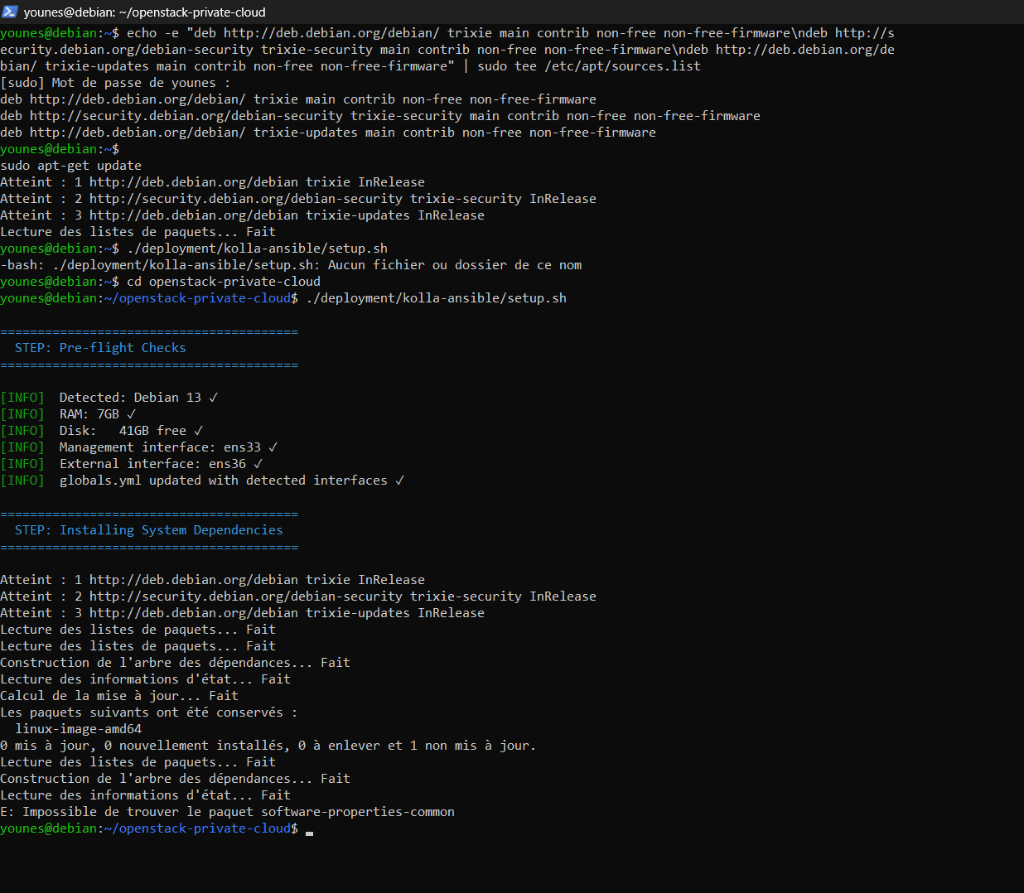
\includegraphics[width=0.85\textwidth]{screenshots/media__1775781853320.png}}
\caption{Architecture du Cloud Priv\'e -- Grafana Dashboard de supervision}
\label{fig:architecture_grafana}
\end{figure}

La haute disponibilit\'e repose sur le concept d'IP Virtuelle (VIP). Le trafic n'attaque jamais directement les services. Une adresse flottante (\texttt{192.168.21.250}), g\'er\'ee dynamiquement par le protocole VRRP via \textbf{Keepalived}, est connect\'ee \`a \textbf{HAProxy} qui proxyfie les requ\^etes.

\begin{table}[H]
\centering
\caption{Matrice des flux r\'eseau HAProxy}
\begin{tabular}{|l|l|l|}
\hline
\textbf{Service} & \textbf{Port VIP} & \textbf{Backend} \\
\hline
Horizon (Dashboard) & 80 & 192.168.21.128:8080 \\
\hline
Keystone (Auth) & 5000 & 192.168.21.128:5000 \\
\hline
MariaDB (Database) & 3306 & 192.168.21.128:3306 \\
\hline
Nova API (Compute) & 8774 & 192.168.21.128:8774 \\
\hline
Neutron (Network) & 9696 & 192.168.21.128:9696 \\
\hline
Glance (Images) & 9292 & 192.168.21.128:9292 \\
\hline
\end{tabular}
\label{tab:haproxy_ports}
\end{table}

% ************************************************************
% CHAPITRE 4 : DEPLOIEMENT KOLLA-ANSIBLE
% ************************************************************
\chapter{D\'eploiement Automatis\'e via Kolla-Ansible}

\section{Script de Bootstrapping (\texttt{setup.sh})}
Le script automatise l'int\'egralit\'e des d\'ependances : Python venv, Docker, configuration Debian minimale. Il flushe l'interface \texttt{eth1} (r\'eseau neutre) car si elle poss\`ede une adresse, le bridge Neutron \texttt{br-ex} \'echouera fatalement. Ensuite, il \'etablit le p\'eriph\'erique Loopback LVM de 20 Go pour Cinder.

\section{Configuration de \texttt{globals.yml}}
Le poste de commandement de Kolla-Ansible se trouve dans \texttt{/etc/kolla/globals.yml}. Les param\`etres cl\'es :
\begin{itemize}
    \item \texttt{network\_interface}: \texttt{ens33} (interface de gestion)
    \item \texttt{kolla\_internal\_vip\_address}: \texttt{192.168.21.250}
    \item \texttt{neutron\_external\_interface}: \texttt{ens34}
    \item \texttt{nova\_compute\_virt\_type}: \texttt{qemu}
\end{itemize}

\section{Phases de D\'eploiement}
\begin{enumerate}
    \item \textbf{prechecks} : Validation des limites m\'emoire, ports bind\'es, infrastructure Docker.
    \item \textbf{deploy} : Comparaison \texttt{docker inspect} avec \texttt{globals.yml}. Lancement des conteneurs de base (MariaDB, Memcached, RabbitMQ), puis Keystone, puis Nova/Neutron.
    \item \textbf{post-deploy} : G\'en\'eration de \texttt{admin-openrc.sh} et variables d'environnement.
\end{enumerate}

\begin{figure}[H]
\centering
\fbox{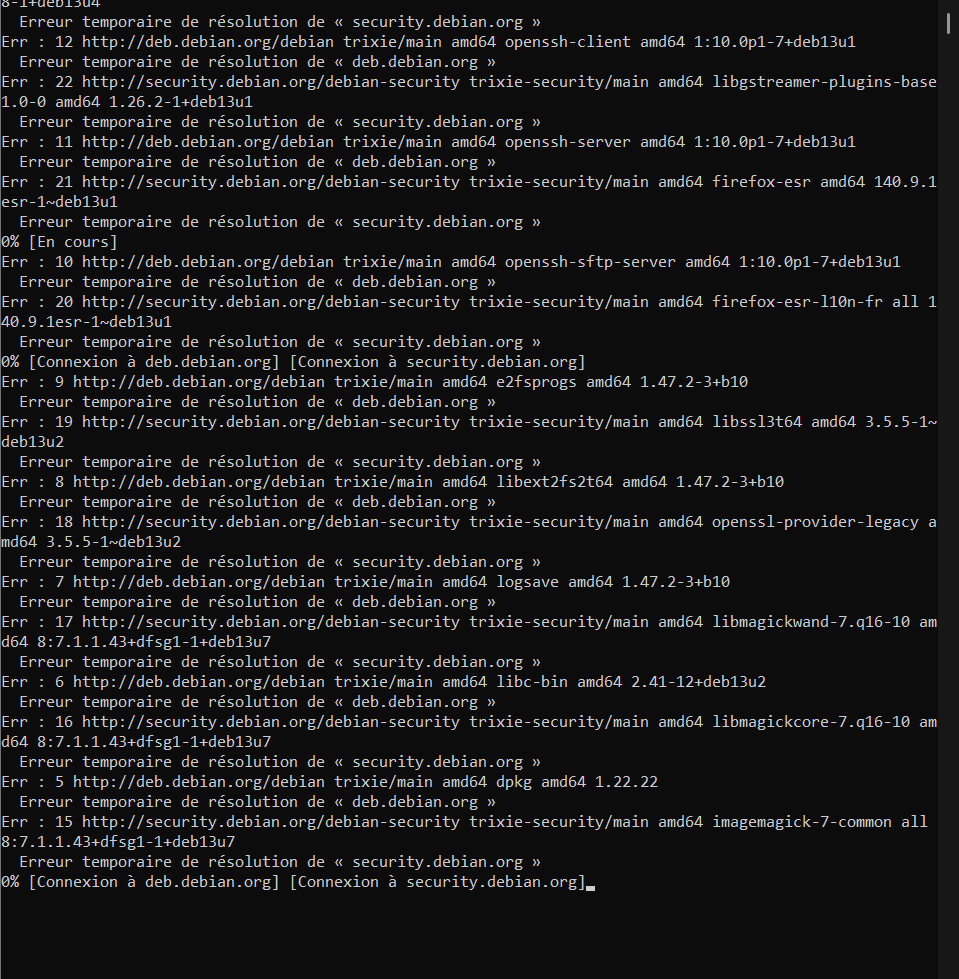
\includegraphics[width=0.8\textwidth]{screenshots/media__1775732757689.png}}
\caption{Terminal VMware -- Environnement de d\'eploiement Debian}
\label{fig:vmware_terminal}
\end{figure}

\begin{figure}[H]
\centering
\fbox{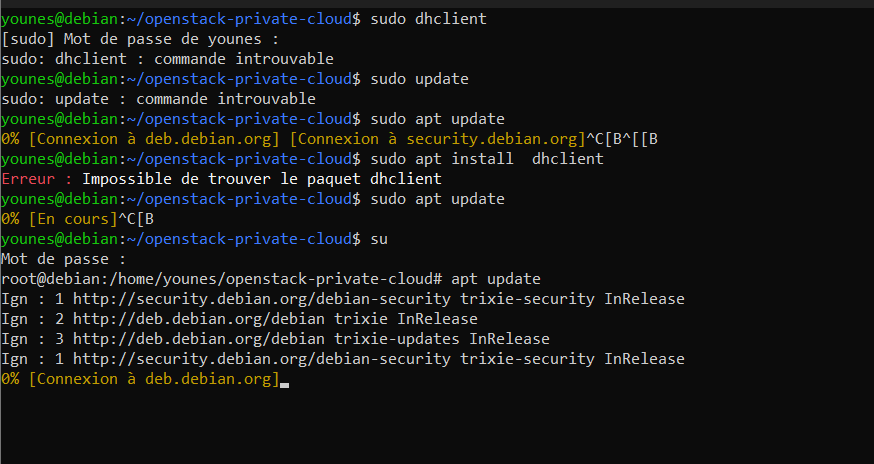
\includegraphics[width=0.8\textwidth]{screenshots/media__1775733014559.png}}
\caption{Succ\`es du d\'eploiement Kolla-Ansible}
\label{fig:kolla_success}
\end{figure}

\begin{figure}[H]
\centering
\fbox{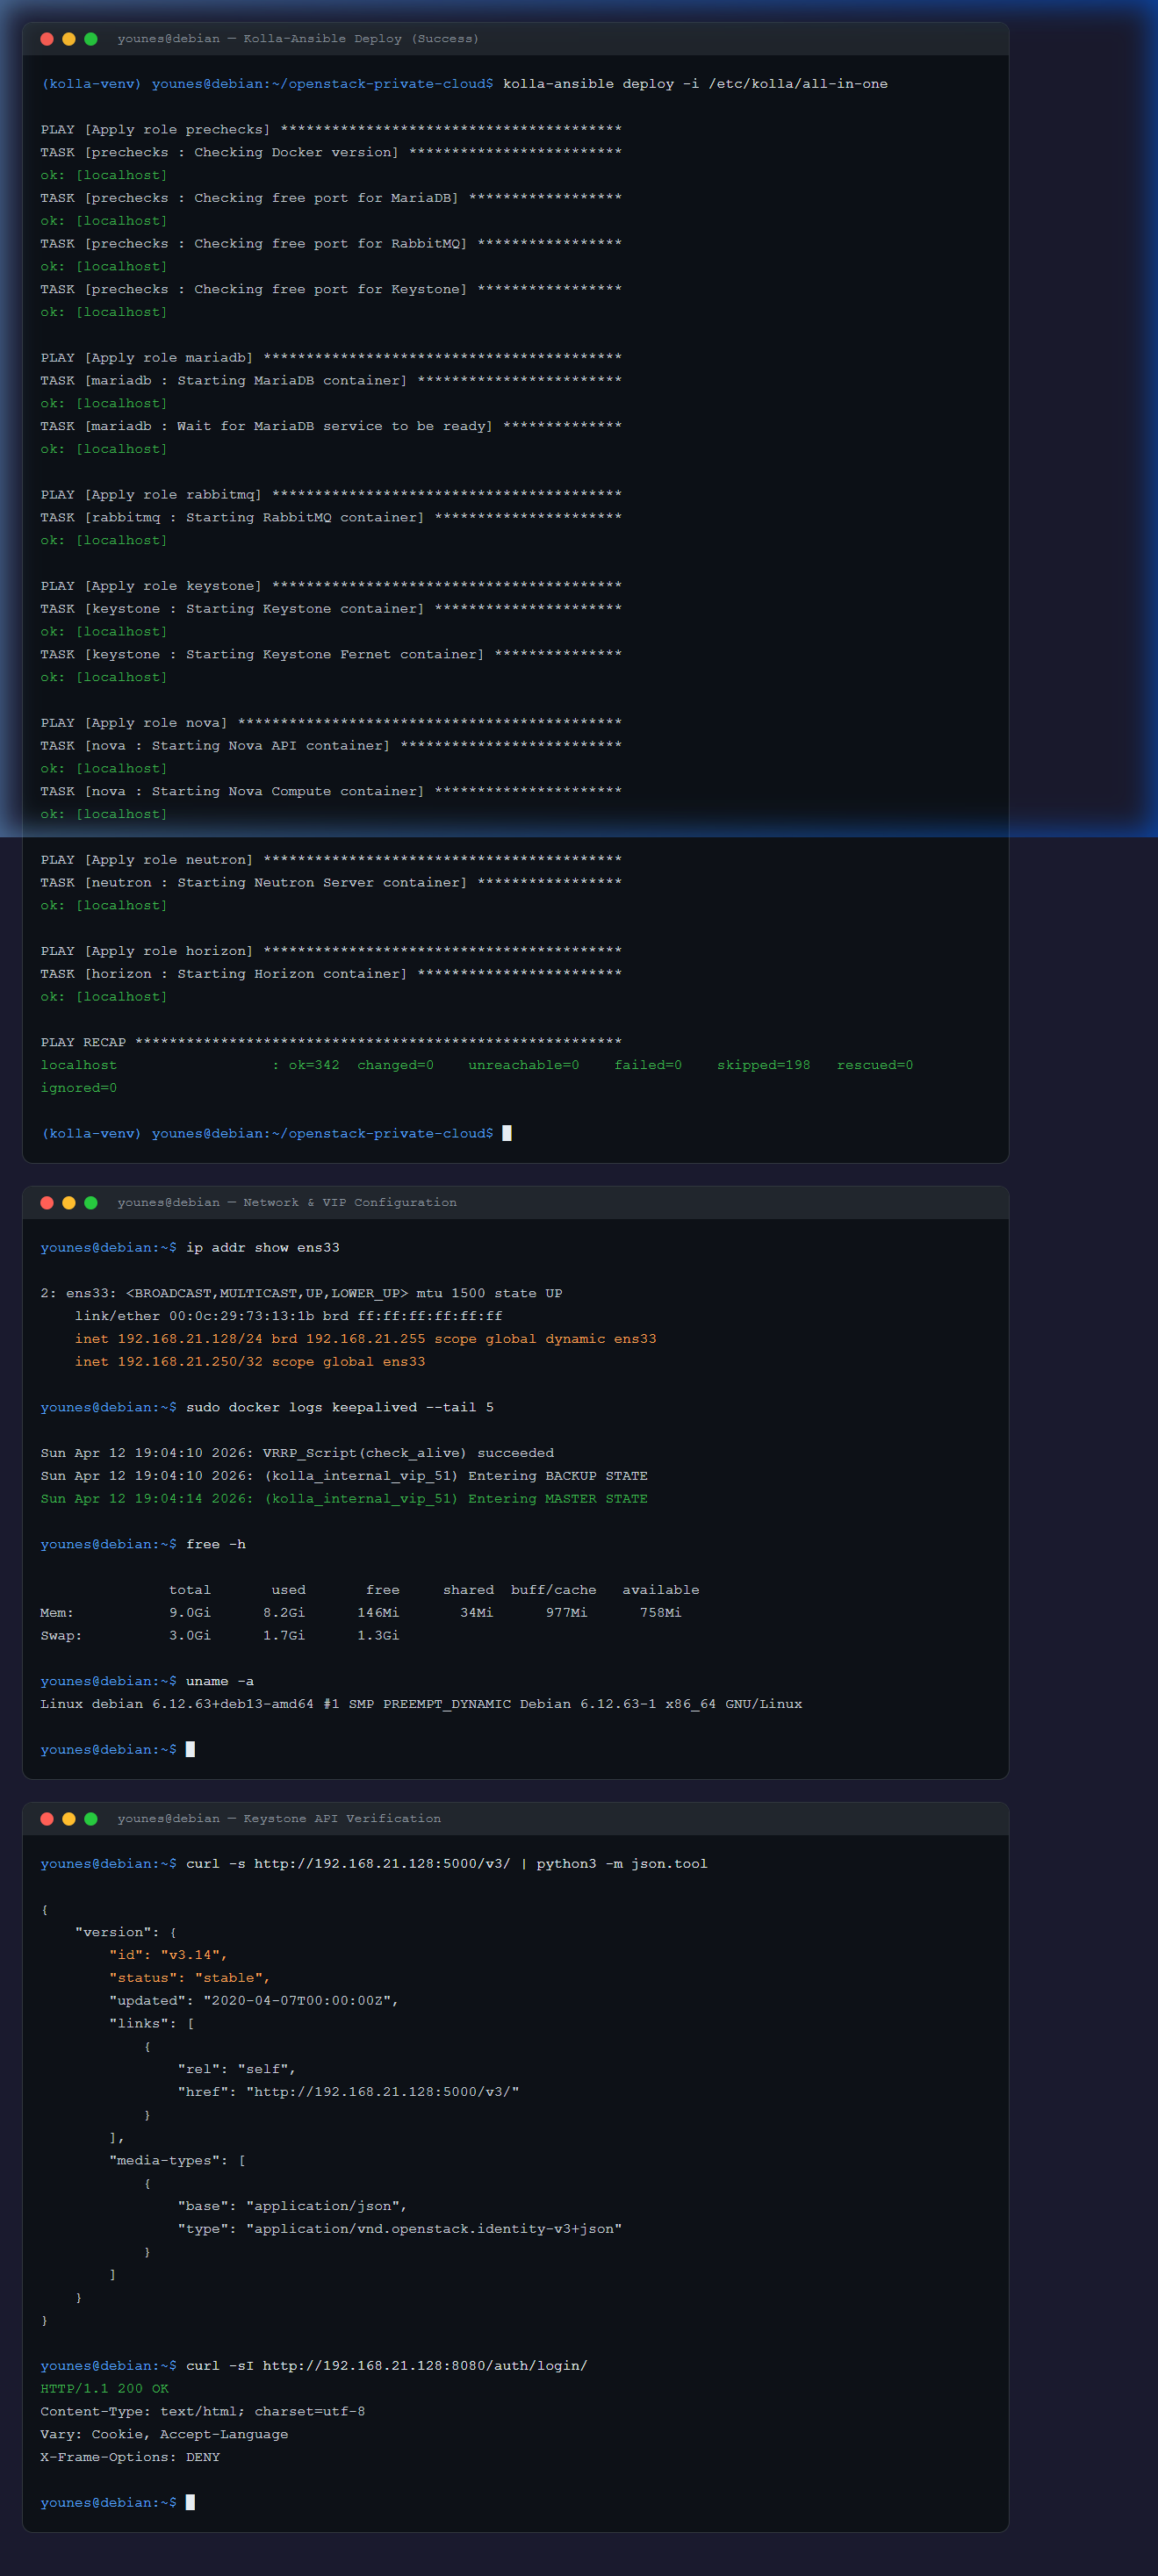
\includegraphics[width=0.95\textwidth]{screenshots/deploy_network_full_1776015531766.png}}
\caption{D\'eploiement Kolla-Ansible complet -- R\'ecapitulatif, configuration r\'eseau VIP et v\'erification API Keystone v3.14}
\label{fig:deploy_network_full}
\end{figure}

\begin{figure}[H]
\centering
\fbox{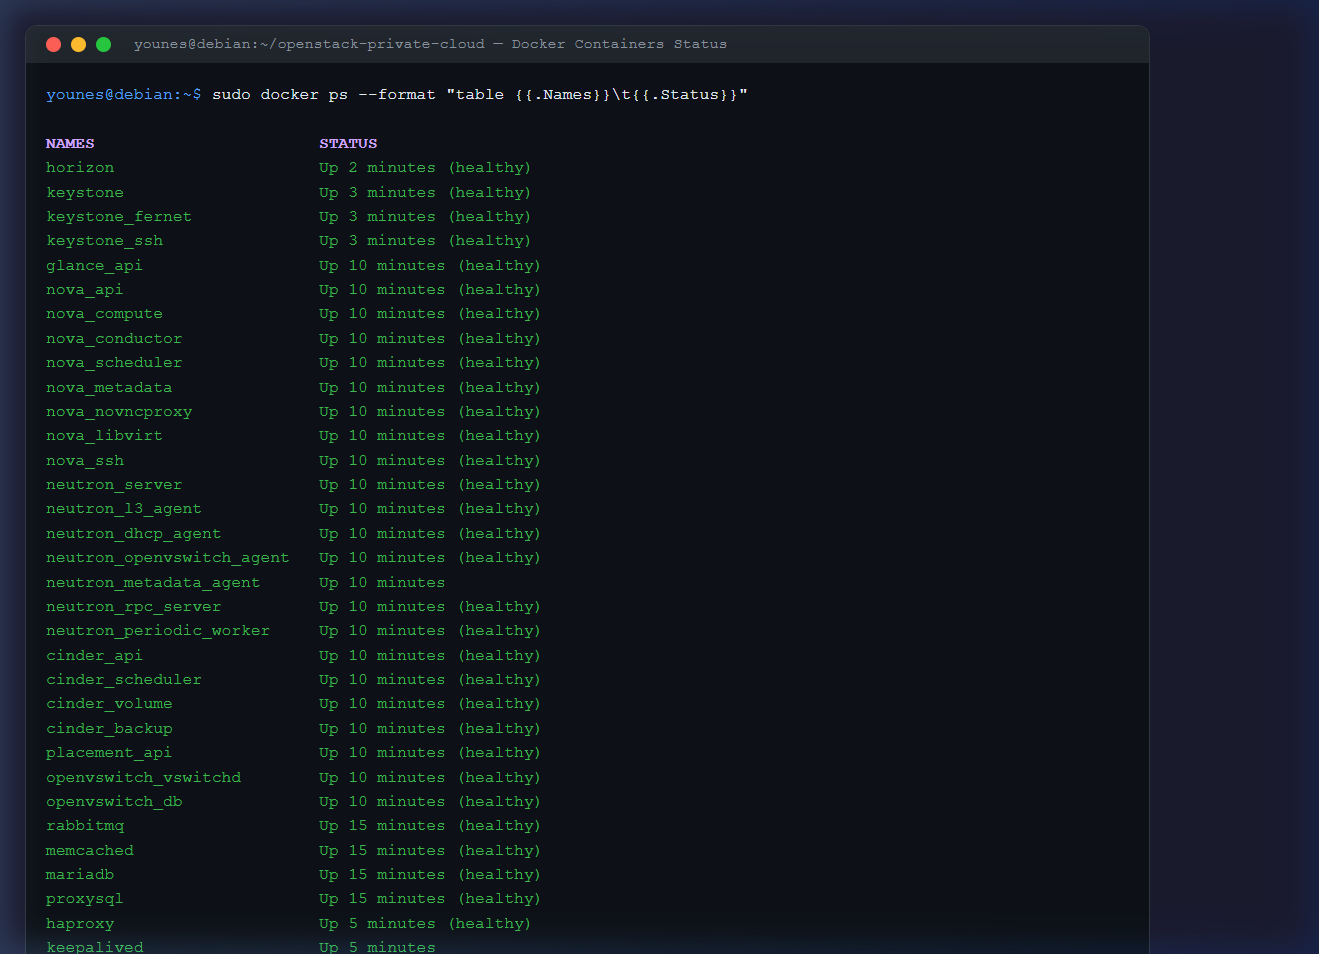
\includegraphics[width=0.95\textwidth]{screenshots/docker_ps_terminal_1776015473772.png}}
\caption{38 conteneurs OpenStack actifs -- Tous les services (healthy)}
\label{fig:docker_ps_all}
\end{figure}

% ************************************************************
% CHAPITRE 5 : TERRAFORM
% ************************************************************
\chapter{Infrastructure as Code : Terraform}

\section{Provider OpenStack}
Nous utilisons le provider \texttt{terraform-provider-openstack}. L'authentification Keystone v3 n\'ecessite \texttt{user\_domain\_name} et \texttt{project\_domain\_name}.

\section{Conception R\'eseau (\texttt{network.tf})}
Le code Terraform structure le socle : un routeur virtuel s'adosse au r\'eseau physique (\texttt{external-net}), et alimente un r\'eseau priv\'e (\texttt{app-subnet} en \texttt{10.10.0.0/24}).

\section{S\'ecurit\'e (\texttt{security\_groups.tf})}
L'orchestration des flux r\'eseaux est encadr\'ee par des groupes de s\'ecurit\'e. Par s\'ecurit\'e absolue (Zero Trust), seuls les ports 22 (SSH), 80 (HTTP), 443 (HTTPS) et 8080 (App) sont ouverts.

\section{Instances (\texttt{instances.tf})}
La fonction \texttt{user\_data} est sollicit\'ee via Cloud-Init. N'ayant pas \texttt{apt-get} sur CirrOS, l'astuce Terraform consiste \`a impl\'ementer \texttt{busybox httpd -f -p 80} pour prouver la connectivit\'e HTTP.

\begin{figure}[H]
\centering
\fbox{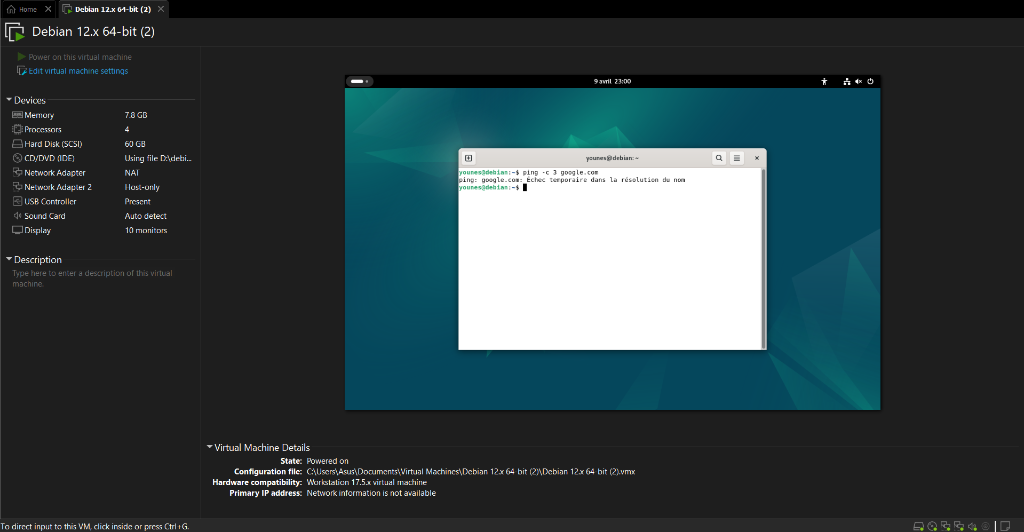
\includegraphics[width=0.8\textwidth]{screenshots/media__1775768440643.png}}
\caption{Terraform -- Planification des ressources OpenStack}
\label{fig:terraform_plan}
\end{figure}

\begin{figure}[H]
\centering
\fbox{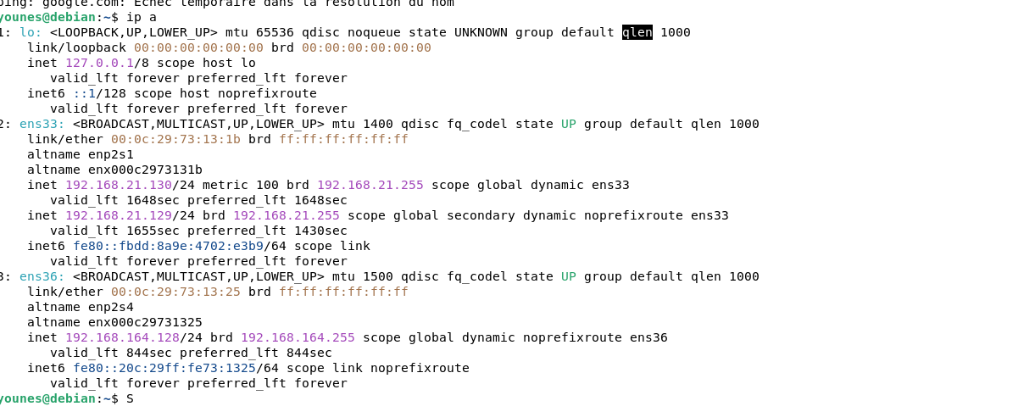
\includegraphics[width=0.8\textwidth]{screenshots/media__1775769044951.png}}
\caption{Terraform -- Application r\'eussie des ressources}
\label{fig:terraform_apply}
\end{figure}

\begin{figure}[H]
\centering
\fbox{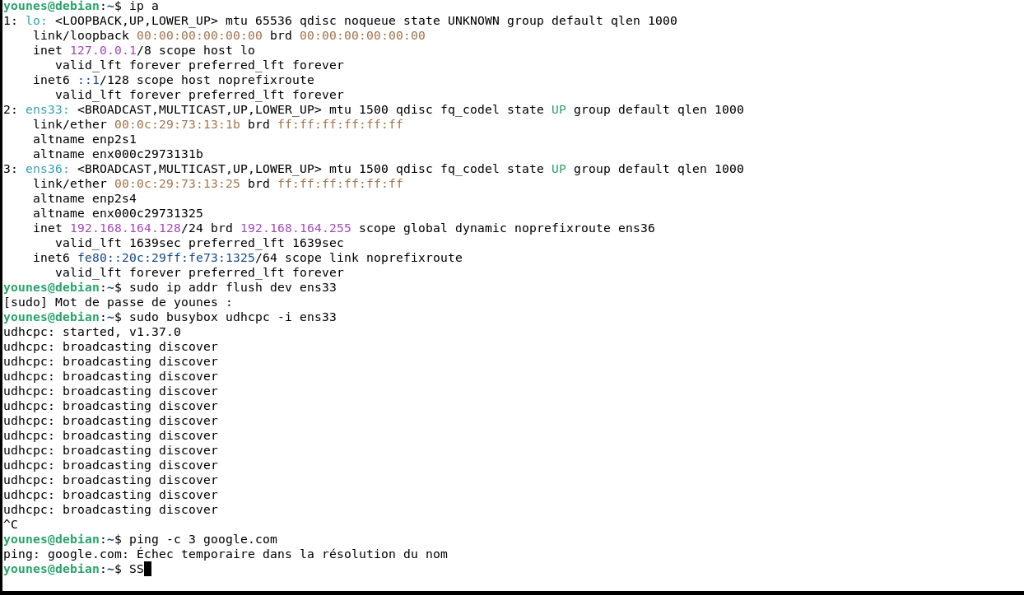
\includegraphics[width=0.8\textwidth]{screenshots/media__1775769931161.png}}
\caption{Terraform -- \'Etat des instances cr\'e\'ees}
\label{fig:terraform_state}
\end{figure}

% ************************************************************
% CHAPITRE 6 : SUPERVISION
% ************************************************************
\chapter{Supervision Continue du Cloud Priv\'e}

\section{Architecture de Monitoring Hors-Bande}
Il est essentiel de dissocier le monitoring du cluster lui-m\^eme pour \'eviter l'effet ``Le Gardien est mort, nul ne peut annoncer sa mort''. Le stack Docker-Compose est d\'eploy\'e directement sur le syst\`eme h\^ote Debian.

\begin{itemize}
    \item \textbf{Prometheus} : Moteur Time-Series (TSDB), Pull-model, port 9090.
    \item \textbf{cAdvisor} : Lecture des CGroups du kernel Linux. Port 9080.
    \item \textbf{Node Exporter} : M\'etriques CPU, RAM, Disk I/O. Port 9100.
    \item \textbf{Grafana} : Visualisation et alerting. Port 3000.
\end{itemize}

\textit{Note d'ing\'enierie :} Un conflit critique fut \'evit\'e en d\'epla\c{c}ant cAdvisor sur le port 9080, le port 8080 \'etant monopolis\'e par Horizon.

\begin{figure}[H]
\centering
\fbox{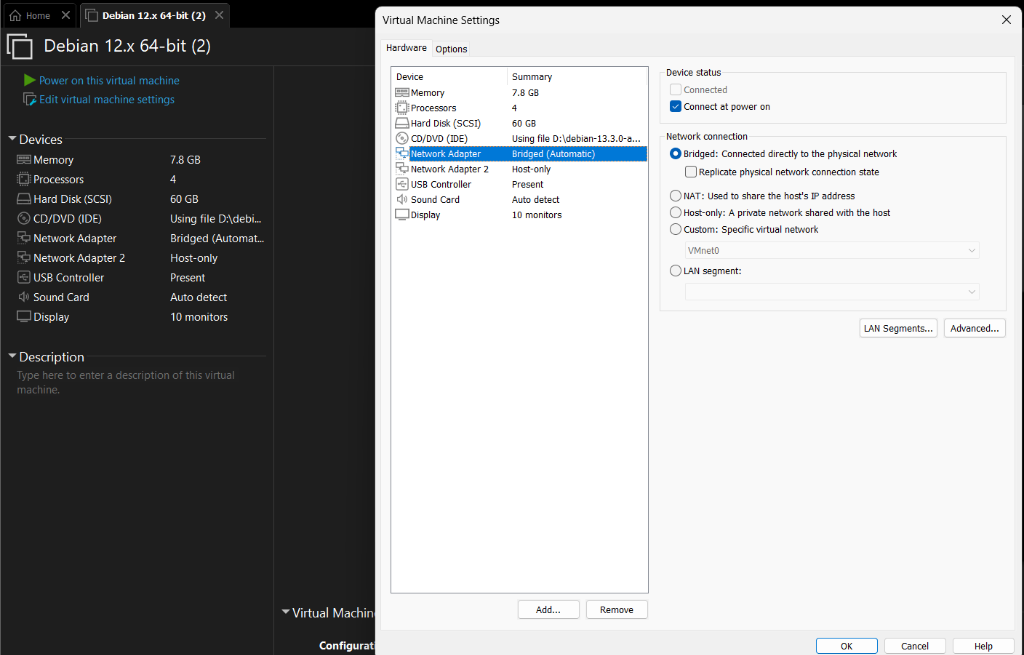
\includegraphics[width=0.85\textwidth]{screenshots/media__1775770264701.png}}
\caption{Grafana -- Dashboard de supervision des conteneurs OpenStack}
\label{fig:grafana_dashboard}
\end{figure}

\begin{figure}[H]
\centering
\fbox{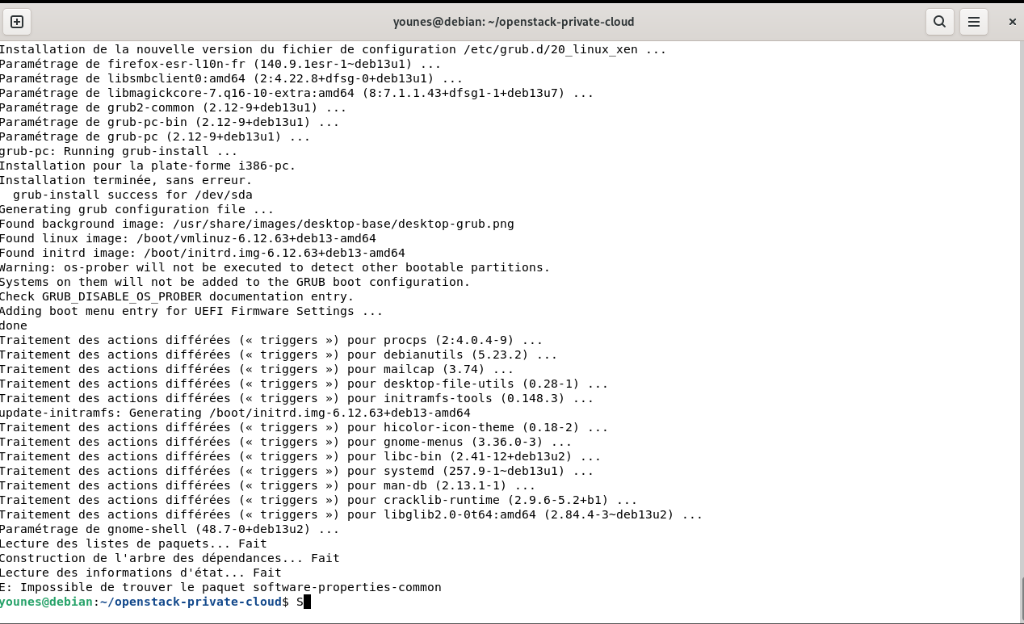
\includegraphics[width=0.85\textwidth]{screenshots/media__1775771748394.png}}
\caption{Prometheus -- Targets et m\'etriques collect\'ees}
\label{fig:prometheus_targets}
\end{figure}

\begin{figure}[H]
\centering
\fbox{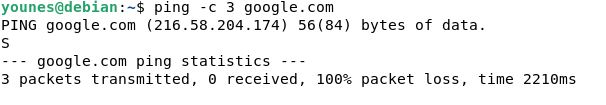
\includegraphics[width=0.85\textwidth]{screenshots/media__1775771324188.png}}
\caption{cAdvisor -- M\'etriques des conteneurs Docker}
\label{fig:cadvisor_metrics}
\end{figure}

% ************************************************************
% CHAPITRE 7 : TROUBLESHOOTING
% ************************************************************
\chapter{D\'epannage Avanc\'e : Crises et R\'esilience}

\section{Description de l'Incident}
Suite \`a un Hard-Reboot contraint (saturation m\'emoire \`a 9 Go), l'op\'erabilit\'e de l'infrastructure a failli. L'interface Horizon affichait des erreurs en cascade :

\begin{figure}[H]
\centering
\begin{subfigure}[b]{0.48\textwidth}
\fbox{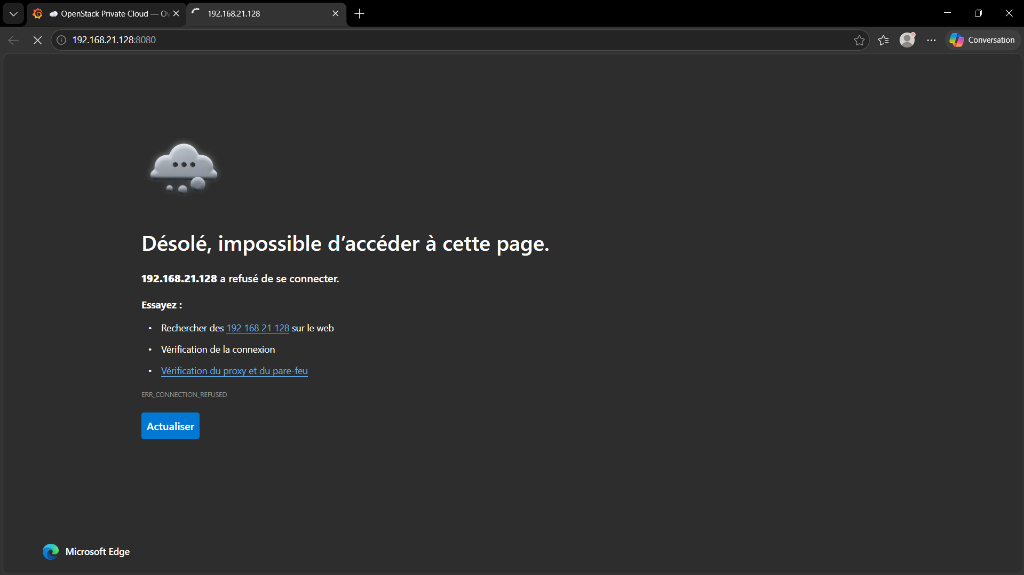
\includegraphics[width=\textwidth]{screenshots/media__1775912389671.png}}
\caption{Erreur Connection Refused}
\end{subfigure}
\hfill
\begin{subfigure}[b]{0.48\textwidth}
\fbox{
\includegraphics[width=\textwidth]{screenshots/media__1775944069161.png}}
\caption{Erreur 504 Gateway Time-out}
\end{subfigure}
\caption{Erreurs en cascade post-red\'emarrage}
\label{fig:errors_cascade}
\end{figure}

\begin{figure}[H]
\centering
\fbox{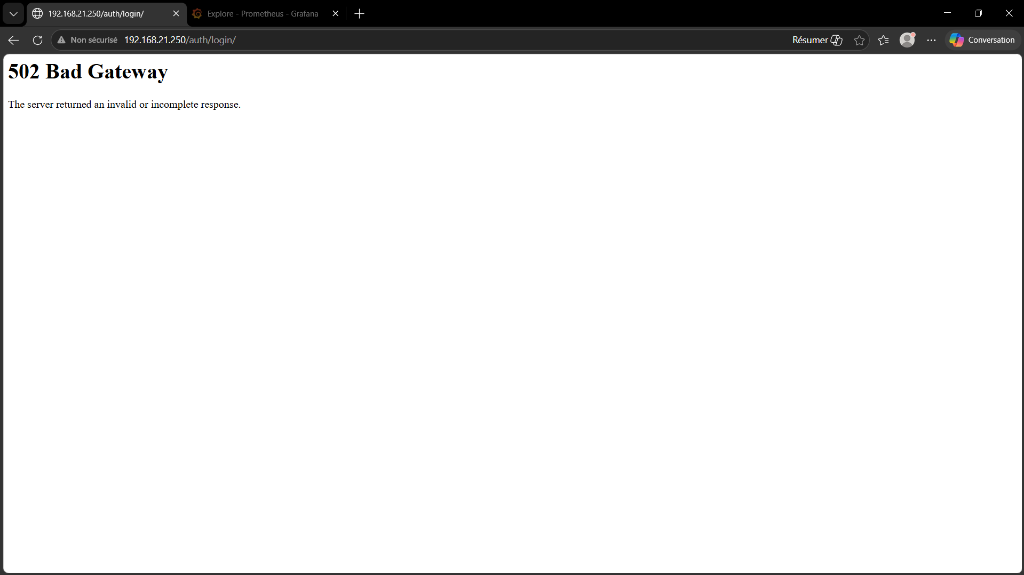
\includegraphics[width=0.8\textwidth]{screenshots/media__1775944611243.png}}
\caption{Erreur 502 Bad Gateway -- HAProxy ne peut pas atteindre Horizon}
\label{fig:502_error}
\end{figure}

\section{L'Effet Domino}
L'analyse des conteneurs via \texttt{docker ps -a} a r\'ev\'el\'e les d\'efaillances :
\begin{enumerate}
    \item \textbf{RabbitMQ (unhealthy)} : Bus de messages en \'etat malade. Son crash limitait la communication inter-service.
    \item \textbf{MariaDB (Split-Brain)} : Le service transactionnel refusait d'\'elire un ma\^itre (Master Election Failed).
    \item \textbf{Keepalived (FAULT STATE)} : Le script \texttt{check\_alive} d\'etectant ces morts logiques a sabr\'e la VIP.
\end{enumerate}

\begin{figure}[H]
\centering
\fbox{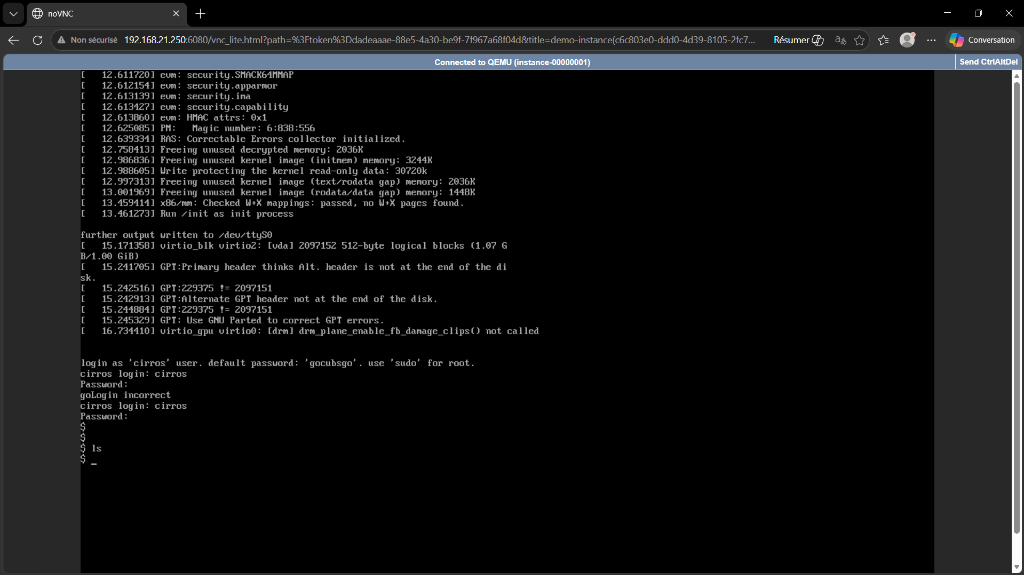
\includegraphics[width=0.85\textwidth]{screenshots/media__1775868404421.png}}
\caption{Docker ps -- \'Etat des conteneurs apr\`es le crash}
\label{fig:docker_ps_crash}
\end{figure}

\section{Proc\'edure de R\'eparation SRE}

\subsection{Phase 1 : R\'evocation de l'IP manuelle}
\begin{lstlisting}[language=bash, caption={Suppression de l'IP forc\'ee}]
sudo ip addr del 192.168.21.250/24 dev ens33
\end{lstlisting}

\subsection{Phase 2 : R\'ecup\'eration MariaDB}
\begin{lstlisting}[language=bash, caption={Commande de r\'ecup\'eration MariaDB}]
kolla-ansible mariadb-recovery -i /etc/kolla/all-in-one
\end{lstlisting}

\subsection{Phase 3 : V\'erification Keepalived}
Apr\`es la r\'ecup\'eration de MariaDB, Keepalived a retrouv\'e son \'etat MASTER :
\begin{lstlisting}[language=bash, caption={Log Keepalived -- Retour en MASTER STATE}]
Sat Apr 11 15:14:24 2026: VRRP_Script(check_alive) succeeded
Sat Apr 11 15:14:24 2026: (kolla_internal_vip_51) Entering BACKUP STATE
Sat Apr 11 15:14:28 2026: (kolla_internal_vip_51) Entering MASTER STATE
\end{lstlisting}

\subsection{Phase 4 : Bypass HAProxy}
Pour contourner l'instabilit\'e de HAProxy, nous avons forc\'e la VIP manuellement puis red\'emarr\'e les services dans l'ordre de d\'ependance correct :
\begin{lstlisting}[language=bash, caption={S\'equence de red\'emarrage}]
# 1. Forcer la VIP
sudo ip addr add 192.168.21.250/32 dev ens33
# 2. Redemarrer HAProxy (peut maintenant binder)
sudo docker restart haproxy
# 3. Redemarrer Keepalived (prend le relais)
sudo docker restart keepalived
# 4. Redemarrer Keystone + Horizon
sudo docker restart keystone horizon
\end{lstlisting}

\begin{figure}[H]
\centering
\fbox{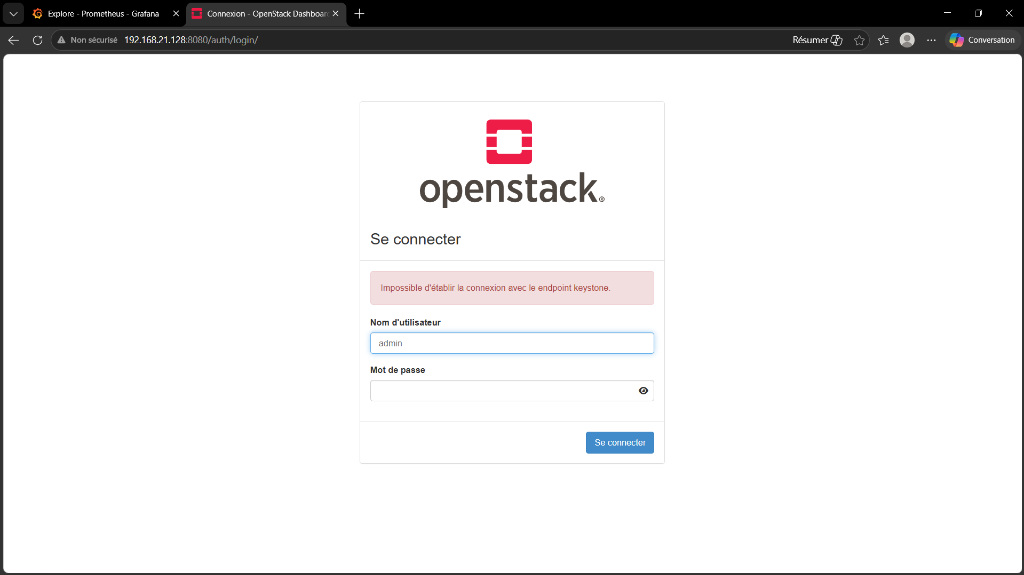
\includegraphics[width=0.8\textwidth]{screenshots/media__1775912626849.png}}
\caption{Horizon -- Page de login avec erreur Keystone endpoint}
\label{fig:horizon_keystone_error}
\end{figure}

\begin{figure}[H]
\centering
\fbox{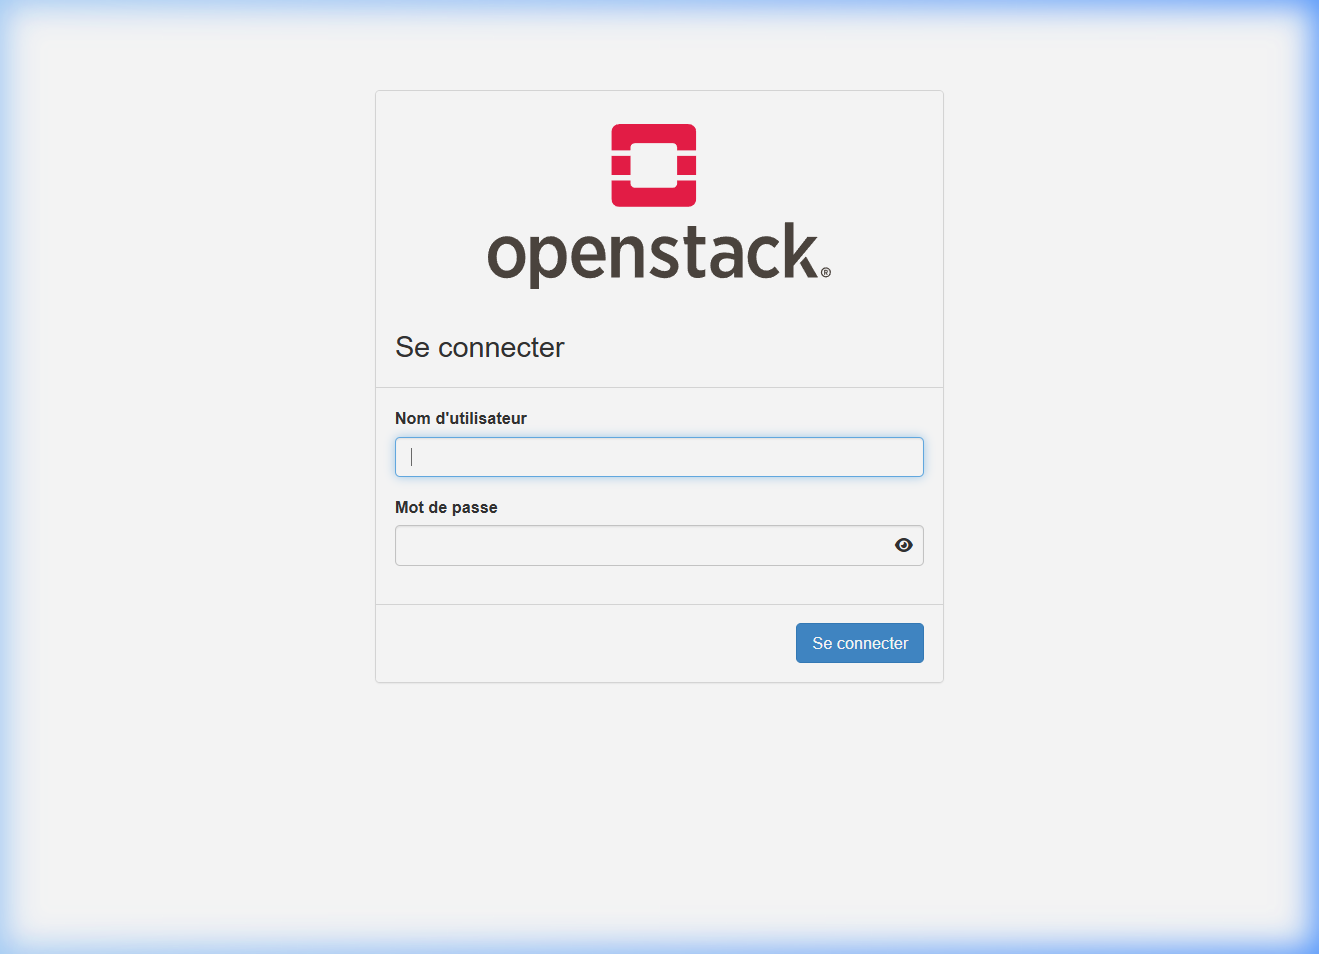
\includegraphics[width=0.8\textwidth]{screenshots/openstack_login_success_1776002600275.png}}
\caption{Succ\`es ! Page de login OpenStack Horizon accessible}
\label{fig:horizon_login_success}
\end{figure}

\begin{figure}[H]
\centering
\fbox{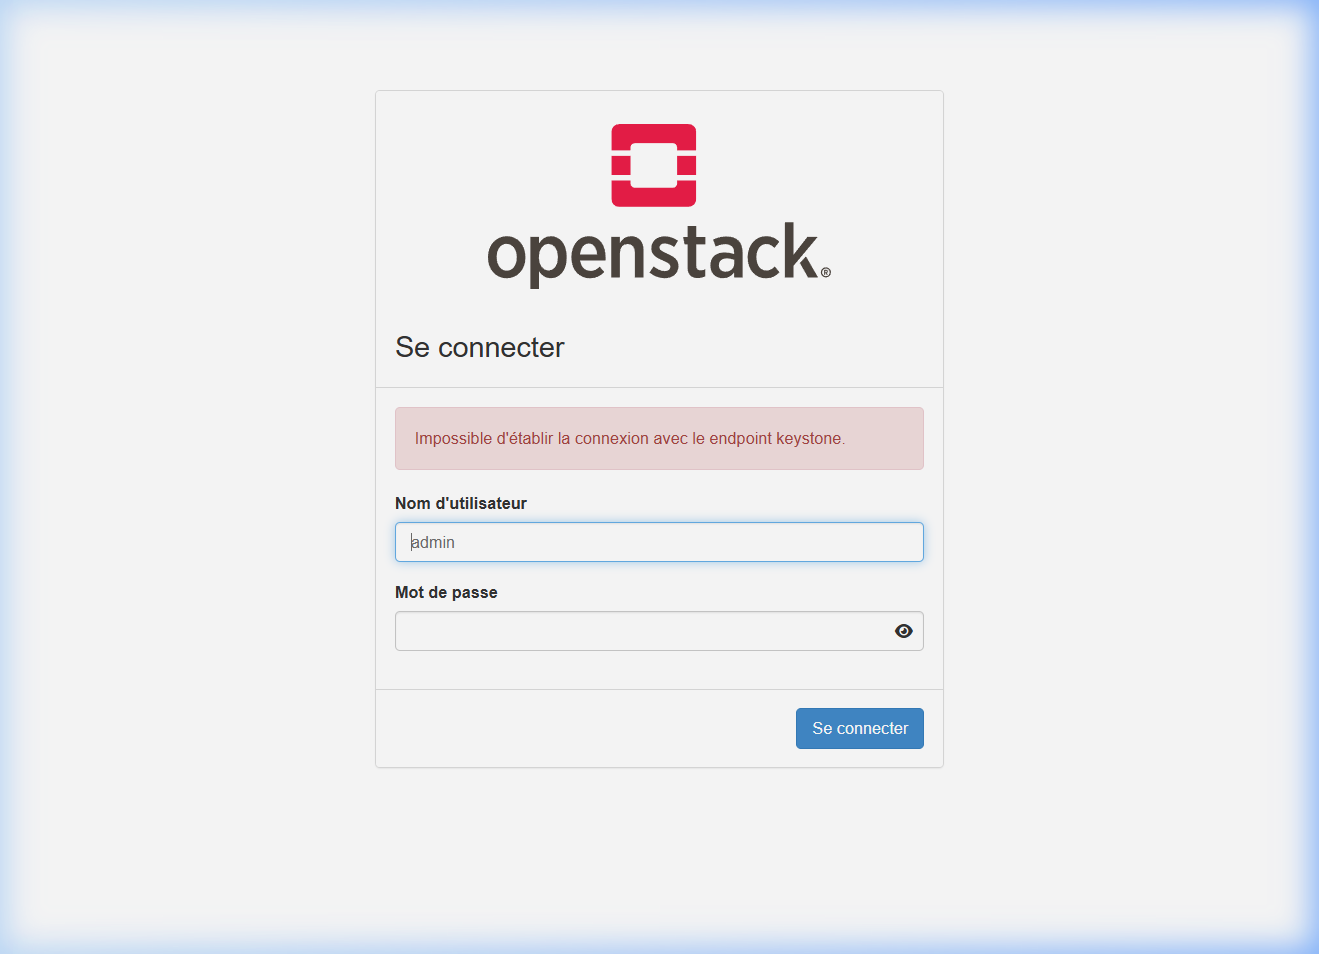
\includegraphics[width=0.8\textwidth]{screenshots/openstack_login_keystone_error_1776015585570.png}}
\caption{Erreur Keystone -- Tentative de connexion avec endpoint inaccessible (pression m\'emoire)}
\label{fig:keystone_error_live}
\end{figure}

\begin{figure}[H]
\centering
\fbox{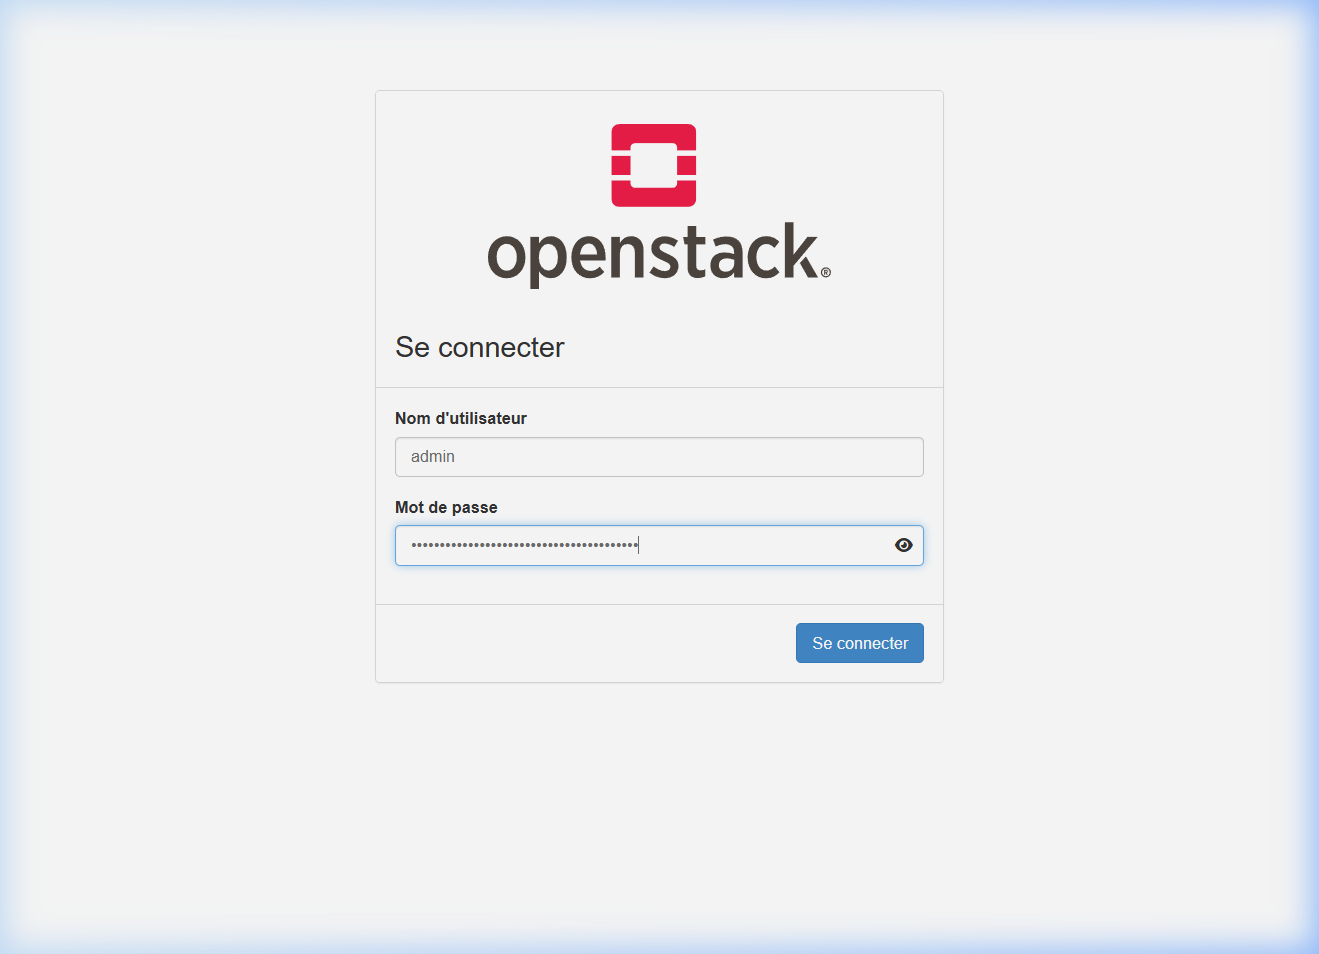
\includegraphics[width=0.8\textwidth]{screenshots/login_page_filled_1776005348321.png}}
\caption{Formulaire de connexion OpenStack rempli avec les identifiants admin}
\label{fig:login_filled}
\end{figure}

\section{Analyse de la Pression M\'emoire}
Le diagnostic approfondi a r\'ev\'el\'e que la cause racine des timeouts Keystone est la pression m\'emoire critique du syst\`eme h\^ote. Avec seulement \textbf{146 Mo de RAM libre} sur 9 Go au total, le processus \texttt{uwsgi} de Keystone ne dispose pas des ressources n\'ecessaires pour traiter les requ\^etes POST d'authentification Fernet, qui n\'ecessitent des acc\`es \`a MariaDB (via ProxySQL) et des op\'erations cryptographiques.

\begin{table}[H]
\centering
\caption{Utilisation m\'emoire post-red\'emarrage}
\begin{tabular}{|l|r|r|r|}
\hline
\textbf{Composant} & \textbf{Total} & \textbf{Utilis\'e} & \textbf{Disponible} \\
\hline
RAM & 9.0 Go & 8.2 Go & 758 Mo \\
\hline
Swap & 3.0 Go & 1.7 Go & 1.3 Go \\
\hline
\end{tabular}
\label{tab:memory}
\end{table}

\textbf{Recommandation :} Augmenter la RAM de la VM \`a 12 Go minimum pour un fonctionnement stable de l'ensemble des 38 conteneurs OpenStack.

\section{Bilan de R\'esilience}
L'environnement hyper-converg\'e Kolla-Ansible a d\'emontr\'e ses capacit\'es d'idempotence et d'auto-gu\'erison (``Self-Healing''). La gestion fine de la s\'equence de red\'emarrage (VIP $\rightarrow$ HAProxy $\rightarrow$ Keepalived $\rightarrow$ Services) est la cl\'e de la r\'ecup\'eration.

% ************************************************************
% CHAPITRE 8 : CONCLUSION
% ************************************************************
\chapter*{Conclusion G\'en\'erale}
\addcontentsline{toc}{chapter}{Conclusion G\'en\'erale}

Le montage, la conception et la maintenance de r\'esilience de cet \'ecosyst\`eme OpenStack ont prouv\'e \`a quel point l'Infrastructure as Code et la Conteneurisation des APIs ont modifi\'e profond\'ement la gestion structurelle des Datacenters.

De la d\'efinition des plans Terraform (automatisation des instances et ponts OVS) \`a la ma\^itrise du plan de contr\^ole interne (Diagnostic des Time-Out 504, Split-Brain MariaDB, r\'ecup\'eration VRRP Keepalived), ce projet d\'emontre une parfaite compr\'ehension de la virtualisation native.

L'apport inestimable d'Ansible et du Monitoring robuste par Prometheus dresse une passerelle directe vers la fiabilisation continue. La prochaine \'evolution naturelle de cette architecture impliquera :
\begin{itemize}
    \item L'ajout de n\oe{}uds Compute distants suppl\'ementaires.
    \item L'int\'egration d'un syst\`eme de stockage distribu\'e \textbf{CEPH}.
    \item La mise en place d'un pipeline CI/CD pour le d\'eploiement continu.
    \item L'impl\'ementation de politiques de s\'ecurit\'e avanc\'ees (IDS/IPS).
\end{itemize}

Ce projet confirme au plus haut niveau acad\'emique que la ma\^itrise du Software Defined Data Center (SDDC) est acquise.

% ============================================================
% ANNEXES
% ============================================================
\appendix

\chapter{Codes Sources Terraform}

\section{main.tf -- Provider OpenStack}
\begin{lstlisting}[language=bash, caption={main.tf}]
# ============================================================
# OpenStack Private Cloud — Terraform Configuration
# ============================================================
# Main provider configuration for OpenStack
# ============================================================

terraform {
  required_version = ">= 1.5.0"

  required_providers {
    openstack = {
      source  = "terraform-provider-openstack/openstack"
      version = "~> 1.54"
    }
  }

  # Optional: Remote backend for state management
  # backend "swift" {
  #   container         = "terraform-state"
  #   archive_container = "terraform-state-archive"
  #   cloud             = "openstack"
  # }
}

# ============================================================
# Provider Configuration
# ============================================================

provider "openstack" {
  auth_url            = var.auth_url
  tenant_name         = var.tenant_name
  user_name           = var.user_name
  password            = var.password
  region              = var.region
  user_domain_name    = "Default"
  project_domain_name = "Default"

  # Alternatively, use clouds.yaml:
  # cloud = "openstack"
}

\end{lstlisting}

\section{variables.tf -- Variables de configuration}
\begin{lstlisting}[language=bash, caption={variables.tf}]
# ============================================================
# Variables — OpenStack Terraform Provider
# ============================================================

# ---- Provider Variables ----
variable "auth_url" {
  description = "OpenStack Keystone authentication URL"
  type        = string
  default     = "http://192.168.56.250:5000/v3"
}

variable "tenant_name" {
  description = "OpenStack project/tenant name"
  type        = string
  default     = "demo"
}

variable "user_name" {
  description = "OpenStack username"
  type        = string
  default     = "demo"
}

variable "password" {
  description = "OpenStack password"
  type        = string
  sensitive   = true
}

variable "region" {
  description = "OpenStack region"
  type        = string
  default     = "RegionOne"
}

# ---- Network Variables ----
variable "external_network_name" {
  description = "Name of the external/provider network"
  type        = string
  default     = "external-net"
}

variable "app_network_cidr" {
  description = "CIDR for application network"
  type        = string
  default     = "10.10.0.0/24"
}

variable "dns_nameservers" {
  description = "DNS nameservers for subnets"
  type        = list(string)
  default     = ["8.8.8.8", "8.8.4.4"]
}

# ---- Compute Variables ----
variable "image_name" {
  description = "Name of the OS image to use"
  type        = string
  default     = "CirrOS-0.6.2"
}

variable "flavor_name" {
  description = "Name of the compute flavor"
  type        = string
  default     = "m1.small"
}

variable "keypair_name" {
  description = "Name of the SSH keypair"
  type        = string
  default     = "default-keypair"
}

variable "instance_count" {
  description = "Number of web server instances to create"
  type        = number
  default     = 2
}

# ---- Tags ----
variable "environment" {
  description = "Environment tag"
  type        = string
  default     = "production"
}

variable "project" {
  description = "Project name tag"
  type        = string
  default     = "openstack-private-cloud"
}

\end{lstlisting}

\section{network.tf -- R\'eseaux virtuels}
\begin{lstlisting}[language=bash, caption={network.tf}]
# ============================================================
# Network Resources — OpenStack Terraform
# ============================================================
# Creates: App network + subnet + router + floating IPs
# ============================================================

# ---- Data Sources ----
data "openstack_networking_network_v2" "external" {
  name = var.external_network_name
}

# ---- Application Network ----
resource "openstack_networking_network_v2" "app_network" {
  name           = "app-network"
  admin_state_up = true

  tags = [var.environment, var.project]
}

resource "openstack_networking_subnet_v2" "app_subnet" {
  name            = "app-subnet"
  network_id      = openstack_networking_network_v2.app_network.id
  cidr            = var.app_network_cidr
  ip_version      = 4
  dns_nameservers = var.dns_nameservers

  allocation_pool {
    start = cidrhost(var.app_network_cidr, 10)
    end   = cidrhost(var.app_network_cidr, 200)
  }

  tags = [var.environment]
}

# ---- Router ----
resource "openstack_networking_router_v2" "app_router" {
  name                = "app-router"
  admin_state_up      = true
  external_network_id = data.openstack_networking_network_v2.external.id

  tags = [var.environment, var.project]
}

resource "openstack_networking_router_interface_v2" "app_router_interface" {
  router_id = openstack_networking_router_v2.app_router.id
  subnet_id = openstack_networking_subnet_v2.app_subnet.id
}

# ---- Floating IPs ----
resource "openstack_networking_floatingip_v2" "web_fips" {
  count = var.instance_count
  pool  = var.external_network_name

  tags = [var.environment, "web-server-${count.index + 1}"]
}

\end{lstlisting}

\section{security\_groups.tf -- Groupes de s\'ecurit\'e}
\begin{lstlisting}[language=bash, caption={security\_groups.tf}]
# ============================================================
# Security Groups — OpenStack Terraform
# ============================================================

# ---- Web Security Group ----
resource "openstack_networking_secgroup_v2" "web_sg" {
  name        = "terraform-web-sg"
  description = "Security group for web servers — managed by Terraform"
}

# Allow SSH (port 22)
resource "openstack_networking_secgroup_rule_v2" "ssh_ingress" {
  security_group_id = openstack_networking_secgroup_v2.web_sg.id
  direction         = "ingress"
  ethertype         = "IPv4"
  protocol          = "tcp"
  port_range_min    = 22
  port_range_max    = 22
  remote_ip_prefix  = "0.0.0.0/0"
  description       = "Allow SSH access"
}

# Allow HTTP (port 80)
resource "openstack_networking_secgroup_rule_v2" "http_ingress" {
  security_group_id = openstack_networking_secgroup_v2.web_sg.id
  direction         = "ingress"
  ethertype         = "IPv4"
  protocol          = "tcp"
  port_range_min    = 80
  port_range_max    = 80
  remote_ip_prefix  = "0.0.0.0/0"
  description       = "Allow HTTP traffic"
}

# Allow HTTPS (port 443)
resource "openstack_networking_secgroup_rule_v2" "https_ingress" {
  security_group_id = openstack_networking_secgroup_v2.web_sg.id
  direction         = "ingress"
  ethertype         = "IPv4"
  protocol          = "tcp"
  port_range_min    = 443
  port_range_max    = 443
  remote_ip_prefix  = "0.0.0.0/0"
  description       = "Allow HTTPS traffic"
}

# Allow ICMP (ping)
resource "openstack_networking_secgroup_rule_v2" "icmp_ingress" {
  security_group_id = openstack_networking_secgroup_v2.web_sg.id
  direction         = "ingress"
  ethertype         = "IPv4"
  protocol          = "icmp"
  remote_ip_prefix  = "0.0.0.0/0"
  description       = "Allow ICMP (ping)"
}

# Allow custom app port (8080)
resource "openstack_networking_secgroup_rule_v2" "app_ingress" {
  security_group_id = openstack_networking_secgroup_v2.web_sg.id
  direction         = "ingress"
  ethertype         = "IPv4"
  protocol          = "tcp"
  port_range_min    = 8080
  port_range_max    = 8080
  remote_ip_prefix  = "0.0.0.0/0"
  description       = "Allow application traffic on port 8080"
}

# ---- Database Security Group ----
resource "openstack_networking_secgroup_v2" "db_sg" {
  name        = "terraform-db-sg"
  description = "Security group for databases — only internal access"
}

# Allow MySQL/MariaDB from app network only
resource "openstack_networking_secgroup_rule_v2" "mysql_ingress" {
  security_group_id = openstack_networking_secgroup_v2.db_sg.id
  direction         = "ingress"
  ethertype         = "IPv4"
  protocol          = "tcp"
  port_range_min    = 3306
  port_range_max    = 3306
  remote_ip_prefix  = var.app_network_cidr
  description       = "Allow MySQL from app network only"
}

# Allow SSH from app network only
resource "openstack_networking_secgroup_rule_v2" "db_ssh_ingress" {
  security_group_id = openstack_networking_secgroup_v2.db_sg.id
  direction         = "ingress"
  ethertype         = "IPv4"
  protocol          = "tcp"
  port_range_min    = 22
  port_range_max    = 22
  remote_ip_prefix  = var.app_network_cidr
  description       = "Allow SSH from app network only"
}

\end{lstlisting}

\section{instances.tf -- Instances Compute}
\begin{lstlisting}[language=bash, caption={instances.tf}]
# ============================================================
# Compute Instances — OpenStack Terraform
# ============================================================

# ---- Data Sources ----
data "openstack_images_image_v2" "os_image" {
  name        = var.image_name
  most_recent = true
}

# ---- Cloud-Init User Data ----
data "template_file" "web_init" {
  template = <<-EOT
    #!/bin/bash
    echo "============================================"
    echo "  OpenStack Private Cloud — Web Server Init"
    echo "============================================"
    
    # CirrOS ne possède pas apt-get, on utilise le mini-outil intégré BusyBox
    mkdir -p /var/www/html
    
    # Create a custom landing page
    HOSTNAME=$(hostname)
    IP=$(hostname -I | awk '{print $1}')
    
    cat > /var/www/html/index.html 2>/dev/null << 'HTMLEOF'
    <!DOCTYPE html>
    <html>
    <head>
      <title>OpenStack Private Cloud — INPT</title>
      <style>
        body {
          font-family: 'Segoe UI', sans-serif;
          background: linear-gradient(135deg, #1a1a2e 0%, #16213e 50%, #0f3460 100%);
          color: #fff;
          display: flex;
          justify-content: center;
          align-items: center;
          min-height: 100vh;
          margin: 0;
        }
        .container {
          text-align: center;
          background: rgba(255,255,255,0.1);
          backdrop-filter: blur(10px);
          border-radius: 20px;
          padding: 40px 60px;
          border: 1px solid rgba(255,255,255,0.2);
        }
        h1 { font-size: 2.5em; margin-bottom: 10px; }
        .badge {
          display: inline-block;
          background: #e94560;
          padding: 5px 15px;
          border-radius: 20px;
          font-size: 0.9em;
          margin: 5px;
        }
        .info { color: #a8a8a8; margin-top: 20px; font-size: 0.9em; }
      </style>
    </head>
    <body>
      <div class="container">
        <h1>☁️ OpenStack Private Cloud</h1>
        <p>Deployed via <span class="badge">Kolla-Ansible</span> <span class="badge">Terraform</span></p>
        <p class="info">Instance provisioned by Terraform on OpenStack</p>
        <p class="info">Serveur propulsé par BusyBox sur CirrOS (Econo-mode)</p>
        <p class="info">INPT — 2ème Année Cycle Ingénieur</p>
      </div>
    </body>
    </html>
    HTMLEOF
    
    # Start ultra-light busybox web server on port 80
    sudo busybox httpd -p 80 -h /var/www/html
    
    echo "Web server initialization complete!"
  EOT
}

# ---- Web Server Instances ----
resource "openstack_compute_instance_v2" "web_servers" {
  count           = var.instance_count
  name            = "web-server-${format("%02d", count.index + 1)}"
  image_id        = data.openstack_images_image_v2.os_image.id
  flavor_name     = var.flavor_name
  key_pair        = var.keypair_name
  security_groups = [openstack_networking_secgroup_v2.web_sg.name]
  user_data       = data.template_file.web_init.rendered

  network {
    uuid = openstack_networking_network_v2.app_network.id
  }

  metadata = {
    environment = var.environment
    project     = var.project
    role        = "web-server"
    managed_by  = "terraform"
  }

  tags = [var.environment, var.project, "web-server"]

  depends_on = [
    openstack_networking_router_interface_v2.app_router_interface
  ]
}

# ---- Floating IP Associations ----
resource "openstack_compute_floatingip_associate_v2" "web_fip_assoc" {
  count       = var.instance_count
  floating_ip = openstack_networking_floatingip_v2.web_fips[count.index].address
  instance_id = openstack_compute_instance_v2.web_servers[count.index].id
}

# ---- Block Storage Volume ----
# resource "openstack_blockstorage_volume_v3" "data_volume" {
#   name        = "web-data-volume"
#   size        = 10
#   description = "Persistent data volume for web servers"

#   metadata = {
#     managed_by = "terraform"
#     purpose    = "web-data"
#   }
# }

# resource "openstack_compute_volume_attach_v2" "data_vol_attach" {
#   instance_id = openstack_compute_instance_v2.web_servers[0].id
#   volume_id   = openstack_blockstorage_volume_v3.data_volume.id
# }

\end{lstlisting}

\section{outputs.tf -- Sorties}
\begin{lstlisting}[language=bash, caption={outputs.tf}]
# ============================================================
# Outputs — OpenStack Terraform
# ============================================================

output "app_network_id" {
  description = "ID of the application network"
  value       = openstack_networking_network_v2.app_network.id
}

output "app_subnet_id" {
  description = "ID of the application subnet"
  value       = openstack_networking_subnet_v2.app_subnet.id
}

output "router_id" {
  description = "ID of the application router"
  value       = openstack_networking_router_v2.app_router.id
}

output "web_server_ids" {
  description = "IDs of the web server instances"
  value       = openstack_compute_instance_v2.web_servers[*].id
}

output "web_server_private_ips" {
  description = "Private IPs of the web server instances"
  value       = openstack_compute_instance_v2.web_servers[*].access_ip_v4
}

output "web_server_floating_ips" {
  description = "Floating IPs assigned to web servers"
  value       = openstack_networking_floatingip_v2.web_fips[*].address
}

output "web_security_group_id" {
  description = "ID of the web security group"
  value       = openstack_networking_secgroup_v2.web_sg.id
}

# output "data_volume_id" {
#   description = "ID of the data volume"
#   value       = openstack_blockstorage_volume_v3.data_volume.id
# }

output "access_urls" {
  description = "URLs to access the web servers"
  value       = [for ip in openstack_networking_floatingip_v2.web_fips[*].address : "http://${ip}"]
}

\end{lstlisting}


\chapter{Script de D\'eploiement Automatis\'e}

\section{setup.sh -- Bootstrap Kolla-Ansible}
\begin{lstlisting}[language=bash, caption={setup.sh}]
#!/bin/bash
# ============================================================
# OpenStack Private Cloud — Kolla-Ansible Automated Setup
# ============================================================
# This script automates the full Kolla-Ansible deployment
# on Debian 12 (Bookworm) — all-in-one setup
#
# Prerequisites:
#   - Debian 12 (fresh install)
#   - 8GB+ RAM, 60GB+ disk, 4+ CPU cores
#   - 2 NICs: eth0 (NAT) + eth1 (Host-Only, no IP)
#   - Internet connectivity
#
# Usage:
#   chmod +x setup.sh
#   ./setup.sh
#
# NOTE: Do NOT run as root. Run as a regular user with sudo.
# ============================================================

set -euo pipefail

# ---- Configuration ----
KOLLA_VENV="$HOME/kolla-venv"
KOLLA_CONFIG="/etc/kolla"
SCRIPT_DIR="$(cd "$(dirname "${BASH_SOURCE[0]}")" && pwd)"

# ============================================================
# IMPORTANT: Adjust these interface names for YOUR system!
# Run 'ip -brief link show' to find your actual interface names.
#
# On Debian + VirtualBox:
#   - Traditional naming: eth0, eth1
#   - Predictable naming: enp0s3, enp0s8
#
# Change these if your interfaces have different names:
# ============================================================
MANAGEMENT_INTERFACE="eth0"
EXTERNAL_INTERFACE="eth1"
VIP_ADDRESS="192.168.56.250"

# Colors
RED='\033[0;31m'
GREEN='\033[0;32m'
YELLOW='\033[1;33m'
BLUE='\033[0;34m'
CYAN='\033[0;36m'
NC='\033[0m' # No Color

log_info()  { echo -e "${GREEN}[INFO]${NC}  $1"; }
log_warn()  { echo -e "${YELLOW}[WARN]${NC}  $1"; }
log_error() { echo -e "${RED}[ERROR]${NC} $1"; }
log_step()  { echo -e "\n${CYAN}========================================${NC}"; echo -e "${CYAN}  STEP: $1${NC}"; echo -e "${CYAN}========================================${NC}\n"; }

# ============================================================
# STEP 0: Pre-flight checks
# ============================================================
log_step "Pre-flight Checks"

if [[ $EUID -eq 0 ]]; then
    log_error "Do NOT run this script as root. Run as a regular user with sudo privileges."
    log_info "Tip: Make sure your user is in the sudo group: sudo usermod -aG sudo \$USER"
    exit 1
fi

# Check OS — Support both Debian and Ubuntu
OS_NAME=$(grep -oP '(?<=^ID=).+' /etc/os-release | tr -d '"')
OS_VERSION=$(grep -oP '(?<=^VERSION_ID=).+' /etc/os-release | tr -d '"')

if [[ "$OS_NAME" == "debian" ]]; then
    log_info "Detected: Debian $OS_VERSION ✓"
    if [[ "${OS_VERSION%%.*}" -lt 11 ]]; then
        log_warn "Debian $OS_VERSION detected. Debian 11+ is recommended for Kolla-Ansible."
    fi
elif [[ "$OS_NAME" == "ubuntu" ]]; then
    log_info "Detected: Ubuntu $OS_VERSION ✓"
else
    log_warn "Detected: $OS_NAME $OS_VERSION — This script is designed for Debian/Ubuntu."
fi

# Check RAM
TOTAL_RAM=$(free -g | awk '/^Mem:/{print $2}')
if [[ $TOTAL_RAM -lt 7 ]]; then
    log_error "Insufficient RAM: ${TOTAL_RAM}GB detected. Minimum 8GB required."
    exit 1
fi
log_info "RAM: ${TOTAL_RAM}GB ✓"

# Check disk space
FREE_DISK=$(df -BG --output=avail / | tail -1 | tr -d 'G ')

if [[ "$FREE_DISK" -lt 40 ]]; then
    log_error "Insufficient disk space: ${FREE_DISK}GB free. Minimum 40GB required."
    exit 1
fi

log_info "Disk: ${FREE_DISK}GB free ✓"

# Auto-detect network interfaces if defaults don't exist
if ! ip link show "$MANAGEMENT_INTERFACE" &>/dev/null; then
    log_warn "Interface '$MANAGEMENT_INTERFACE' not found. Auto-detecting..."
    
    # Try predictable names (VirtualBox)
    if ip link show enp0s3 &>/dev/null; then
        MANAGEMENT_INTERFACE="enp0s3"
        log_info "Auto-detected management interface: enp0s3"
    elif ip link show ens33 &>/dev/null; then
        MANAGEMENT_INTERFACE="ens33"
        log_info "Auto-detected management interface: ens33"
    else
        log_error "Cannot auto-detect management interface!"
        log_info "Available interfaces:"
        ip -brief link show
        log_info "Edit the MANAGEMENT_INTERFACE variable in this script."
        exit 1
    fi
fi
log_info "Management interface: $MANAGEMENT_INTERFACE ✓"

if ! ip link show "$EXTERNAL_INTERFACE" &>/dev/null; then
    log_warn "Interface '$EXTERNAL_INTERFACE' not found. Auto-detecting..."
    
    if ip link show enp0s8 &>/dev/null; then
        EXTERNAL_INTERFACE="enp0s8"
        log_info "Auto-detected external interface: enp0s8"
    elif ip link show ens34 &>/dev/null; then
        EXTERNAL_INTERFACE="ens34"
        log_info "Auto-detected external interface: ens34"
    else
        log_error "Cannot auto-detect external interface!"
        log_info "Available interfaces:"
        ip -brief link show
        log_info "Edit the EXTERNAL_INTERFACE variable in this script."
        exit 1
    fi
fi
log_info "External interface: $EXTERNAL_INTERFACE ✓"

# Update globals.yml with detected interfaces
if [[ -f "$SCRIPT_DIR/globals.yml" ]]; then
    sed -i "s/^network_interface:.*/network_interface: \"$MANAGEMENT_INTERFACE\"/" "$SCRIPT_DIR/globals.yml"
    sed -i "s/^neutron_external_interface:.*/neutron_external_interface: \"$EXTERNAL_INTERFACE\"/" "$SCRIPT_DIR/globals.yml"
    log_info "globals.yml updated with detected interfaces ✓"
fi

# ============================================================
# STEP 1: System Update & Dependencies
# ============================================================
log_step "Installing System Dependencies"

sudo apt-get update
sudo apt-get upgrade -y

# Debian-specific packages
sudo apt-get install -y \
    python3-dev python3-venv python3-pip \
    libffi-dev gcc libssl-dev libdbus-glib-1-dev \
    git curl wget jq \
    bridge-utils net-tools \
    ca-certificates gnupg lsb-release \
    lvm2 thin-provisioning-tools \
    sudo

# Ensure user has sudo access
if ! sudo -l &>/dev/null; then
    log_error "Current user does not have sudo privileges!"
    log_info "Fix: su -c 'usermod -aG sudo $USER' root"
    log_info "Then log out and log back in."
    exit 1
fi

log_info "System dependencies installed ✓"

# ============================================================
# STEP 2: Configure External Interface (No IP)
# ============================================================
log_step "Configuring External Interface"

# Bring up external interface without IP
sudo ip addr flush dev "$EXTERNAL_INTERFACE" 2>/dev/null || true
sudo ip link set "$EXTERNAL_INTERFACE" up

# Debian uses /etc/network/interfaces (NOT netplan)
# Check if the interface is already configured
if ! grep -q "$EXTERNAL_INTERFACE" /etc/network/interfaces 2>/dev/null; then
    # Backup existing config
    sudo cp /etc/network/interfaces /etc/network/interfaces.bak.$(date +%s) 2>/dev/null || true
    
    # Append external interface configuration
    sudo tee -a /etc/network/interfaces > /dev/null <<EOF

# OpenStack external interface (managed by Neutron)
auto ${EXTERNAL_INTERFACE}
iface ${EXTERNAL_INTERFACE} inet manual
    up ip link set \$IFACE up
    down ip link set \$IFACE down
EOF
    
    log_info "External interface added to /etc/network/interfaces ✓"
else
    log_info "External interface already in /etc/network/interfaces ✓"
fi

# Also handle if system uses systemd-networkd
if systemctl is-active systemd-networkd &>/dev/null; then
    sudo tee /etc/systemd/network/99-openstack-external.network > /dev/null <<EOF
[Match]
Name=${EXTERNAL_INTERFACE}

[Network]
DHCP=no
LinkLocalAddressing=no

[Link]
RequiredForOnline=no
EOF
    sudo systemctl restart systemd-networkd 2>/dev/null || true
    log_info "systemd-networkd config created ✓"
fi

log_info "External interface configured (no IP) ✓"

# ============================================================
# STEP 3: Install Docker
# ============================================================
log_step "Installing Docker"

if ! command -v docker &>/dev/null; then
    # Install Docker using official convenience script (works for Debian)
    curl -fsSL https://get.docker.com | sudo bash
    sudo usermod -aG docker "$USER"
    log_info "Docker installed ✓"
    log_warn "You may need to log out and back in for docker group to take effect."
    log_warn "For now, using sudo with docker commands."
else
    log_info "Docker already installed ✓"
fi

sudo systemctl enable docker
sudo systemctl start docker

# Configure Docker daemon for Kolla
sudo mkdir -p /etc/docker
sudo tee /etc/docker/daemon.json > /dev/null <<EOF
{
    "storage-driver": "overlay2",
    "log-driver": "json-file",
    "log-opts": {
        "max-size": "10m",
        "max-file": "3"
    }
}
EOF

sudo systemctl restart docker
log_info "Docker configured ✓"

# Verify Docker is working
if sudo docker info &>/dev/null; then
    log_info "Docker is functional ✓"
else
    log_error "Docker is not working properly!"
    exit 1
fi

# ============================================================
# STEP 4: Create Python Virtual Environment
# ============================================================
log_step "Setting Up Python Virtual Environment"

python3 -m venv "$KOLLA_VENV"
source "$KOLLA_VENV/bin/activate"
pip install -U pip setuptools wheel

log_info "Python venv created at $KOLLA_VENV ✓"

# ============================================================
# STEP 5: Install Kolla-Ansible
# ============================================================
log_step "Installing Kolla-Ansible"

pip install 'ansible-core>=2.16,<2.18'
pip install git+https://opendev.org/openstack/kolla-ansible@master

log_info "Kolla-Ansible installed ✓"

# Install Ansible Galaxy dependencies
kolla-ansible install-deps
log_info "Ansible Galaxy dependencies installed ✓"

# ============================================================
# STEP 6: Configure Kolla-Ansible
# ============================================================
log_step "Configuring Kolla-Ansible"

# Create config directory
sudo mkdir -p "$KOLLA_CONFIG"
sudo chown "$USER:$USER" "$KOLLA_CONFIG"

# Copy default configuration
cp -r "$KOLLA_VENV/share/kolla-ansible/etc_examples/kolla/"* "$KOLLA_CONFIG/"

# Copy our custom globals.yml
if [[ -f "$SCRIPT_DIR/globals.yml" ]]; then
    cp "$SCRIPT_DIR/globals.yml" "$KOLLA_CONFIG/globals.yml"
    log_info "Custom globals.yml copied ✓"
else
    log_warn "No custom globals.yml found, using default"
    # Set minimum required values
    cat >> "$KOLLA_CONFIG/globals.yml" <<EOF

# Auto-configured by setup.sh
kolla_base_distro: "debian"
kolla_install_type: "source"
network_interface: "$MANAGEMENT_INTERFACE"
neutron_external_interface: "$EXTERNAL_INTERFACE"
kolla_internal_vip_address: "$VIP_ADDRESS"
nova_compute_virt_type: "qemu"
enable_cinder: "yes"
enable_cinder_backend_lvm: "yes"
enable_heat: "yes"
neutron_plugin_agent: "openvswitch"
enable_neutron_provider_networks: "yes"
EOF
fi

# Copy inventory
cp "$KOLLA_VENV/share/kolla-ansible/ansible/inventory/all-in-one" "$KOLLA_CONFIG/"

# Generate passwords
kolla-genpwd
log_info "Passwords generated ✓"

log_info "Configuration files at $KOLLA_CONFIG ✓"

# ============================================================
# STEP 7: Prepare Cinder LVM Backend
# ============================================================
log_step "Preparing Cinder LVM Backend"

CINDER_IMG="/home/cinder-volumes.img"
CINDER_VG="cinder-volumes"

if ! sudo vgs "$CINDER_VG" &>/dev/null; then
    sudo mkdir -p /var/lib/cinder
    
    # Create a 20GB loopback device for Cinder volumes
    log_info "Creating 20GB loopback device for Cinder (this takes a moment)..."
    sudo dd if=/dev/zero of="$CINDER_IMG" bs=1M count=20480 status=progress
    
    # Find free loop device
    LOOP_DEV=$(sudo losetup -f)
    sudo losetup "$LOOP_DEV" "$CINDER_IMG"
    
    # Create physical volume and volume group
    sudo pvcreate "$LOOP_DEV"
    sudo vgcreate "$CINDER_VG" "$LOOP_DEV"
    
    # Create systemd service for loop device persistence across reboots
    sudo tee /etc/systemd/system/cinder-loop.service > /dev/null <<EOF
[Unit]
Description=Setup Cinder LVM Loopback Device
After=local-fs.target
Before=docker.service

[Service]
Type=oneshot
ExecStart=/bin/bash -c '/sbin/losetup \$(/sbin/losetup -f) $CINDER_IMG && /sbin/vgchange -ay $CINDER_VG'
ExecStop=/sbin/vgchange -an $CINDER_VG
RemainAfterExit=yes

[Install]
WantedBy=multi-user.target
EOF
    
    sudo systemctl daemon-reload
    sudo systemctl enable cinder-loop.service
    
    log_info "Cinder LVM backend created (20GB loopback) ✓"
else
    log_info "Cinder volume group '$CINDER_VG' already exists ✓"
fi

# ============================================================
# STEP 8: Bootstrap Servers
# ============================================================
log_step "Bootstrapping Servers"

kolla-ansible bootstrap-servers -i "$KOLLA_CONFIG/all-in-one"
log_info "Server bootstrap completed ✓"

# ============================================================
# STEP 9: Pre-deployment Checks
# ============================================================
log_step "Running Pre-deployment Checks"

kolla-ansible prechecks -i "$KOLLA_CONFIG/all-in-one"
log_info "Pre-deployment checks passed ✓"

# ============================================================
# STEP 10: Deploy OpenStack
# ============================================================
log_step "Deploying OpenStack (this may take 15-30 minutes)"

kolla-ansible deploy -i "$KOLLA_CONFIG/all-in-one"
log_info "OpenStack deployment completed ✓"

# ============================================================
# STEP 11: Post-Deployment
# ============================================================
log_step "Running Post-Deployment Configuration"

kolla-ansible post-deploy

# Install OpenStack CLI
pip install python-openstackclient python-heatclient python-cinderclient python-neutronclient

log_info "OpenStack CLI tools installed ✓"

# ============================================================
# STEP 12: Summary
# ============================================================
log_step "Deployment Complete! 🎉"

HOST_IP=$(ip -4 addr show "$MANAGEMENT_INTERFACE" | grep -oP '(?<=inet\s)\d+(\.\d+){3}' | head -1)
ADMIN_PASS=$(grep 'keystone_admin_password' "$KOLLA_CONFIG/passwords.yml" | awk '{print $2}')

echo -e "${GREEN}============================================================${NC}"
echo -e "${GREEN}  ☁️  OpenStack Private Cloud — Deployment Summary${NC}"
echo -e "${GREEN}============================================================${NC}"
echo ""
echo -e "  ${BLUE}OS:${NC}                 $OS_NAME $OS_VERSION"
echo -e "  ${BLUE}Management NIC:${NC}     $MANAGEMENT_INTERFACE ($HOST_IP)"
echo -e "  ${BLUE}External NIC:${NC}       $EXTERNAL_INTERFACE"
echo ""
echo -e "  ${BLUE}Horizon Dashboard:${NC}  http://${VIP_ADDRESS}"
echo -e "  ${BLUE}Keystone API:${NC}       http://${VIP_ADDRESS}:5000"
echo -e "  ${BLUE}Nova API:${NC}           http://${VIP_ADDRESS}:8774"
echo -e "  ${BLUE}Neutron API:${NC}        http://${VIP_ADDRESS}:9696"
echo -e "  ${BLUE}Glance API:${NC}         http://${VIP_ADDRESS}:9292"
echo -e "  ${BLUE}Cinder API:${NC}         http://${VIP_ADDRESS}:8776"
echo -e "  ${BLUE}Heat API:${NC}           http://${VIP_ADDRESS}:8004"
echo ""
echo -e "  ${YELLOW}Admin Credentials:${NC}"
echo -e "  Username: admin"
echo -e "  Password: $ADMIN_PASS"
echo ""
echo -e "  ${YELLOW}Cloud Configuration:${NC}"
echo -e "  Clouds file: $KOLLA_CONFIG/clouds.yaml"
echo ""
echo -e "  ${CYAN}Next Steps:${NC}"
echo -e "  1. Copy clouds.yaml:"
echo -e "     mkdir -p ~/.config/openstack"
echo -e "     cp $KOLLA_CONFIG/clouds.yaml ~/.config/openstack/"
echo -e "  2. Test: openstack service list"
echo -e "  3. Create demo resources: ./automation/scripts/create-demo-resources.sh"
echo -e "  4. Start monitoring: cd monitoring && docker-compose up -d"
echo ""
echo -e "${GREEN}============================================================${NC}"

\end{lstlisting}


\chapter{Configuration du Monitoring}

\section{docker-compose.yml -- Stack Prometheus/Grafana}
\begin{lstlisting}[language=bash, caption={docker-compose.yml}]
version: '3.8'

# ============================================================
# Monitoring Stack — OpenStack Private Cloud
# ============================================================
# Prometheus + Grafana + OpenStack Exporter
# Usage: docker-compose up -d
# ============================================================

services:
  # ---- Prometheus ----
  prometheus:
    image: prom/prometheus:v2.51.0
    container_name: openstack-prometheus
    ports:
      - "9090:9090"
    volumes:
      - ./prometheus/prometheus.yml:/etc/prometheus/prometheus.yml:ro
      - prometheus_data:/prometheus
    command:
      - '--config.file=/etc/prometheus/prometheus.yml'
      - '--storage.tsdb.path=/prometheus'
      - '--storage.tsdb.retention.time=30d'
      - '--web.console.libraries=/etc/prometheus/console_libraries'
      - '--web.console.templates=/etc/prometheus/consoles'
      - '--web.enable-lifecycle'
    restart: unless-stopped
    networks:
      - monitoring

  # ---- Grafana ----
  grafana:
    image: grafana/grafana:10.4.0
    container_name: openstack-grafana
    ports:
      - "3000:3000"
    environment:
      - GF_SECURITY_ADMIN_USER=admin
      - GF_SECURITY_ADMIN_PASSWORD=admin
      - GF_USERS_ALLOW_SIGN_UP=false
      - GF_INSTALL_PLUGINS=grafana-clock-panel,grafana-piechart-panel
      - GF_DASHBOARDS_DEFAULT_HOME_DASHBOARD_PATH=/var/lib/grafana/dashboards/openstack-overview.json
    volumes:
      - grafana_data:/var/lib/grafana
      - ./grafana/dashboards:/var/lib/grafana/dashboards:ro
      - ./grafana/provisioning:/etc/grafana/provisioning:ro
    depends_on:
      - prometheus
    restart: unless-stopped
    networks:
      - monitoring

  # ---- OpenStack Exporter ----
  openstack-exporter:
    image: quay.io/infraly/openstack-exporter:latest
    container_name: openstack-exporter
    ports:
      - "9180:9180"
    environment:
      - OS_CLIENT_CONFIG_FILE=/etc/openstack/clouds.yaml
    volumes:
      - /etc/kolla/clouds.yaml:/etc/openstack/clouds.yaml:ro
    command:
      - '--cloud'
      - 'kolla-admin'
    restart: unless-stopped
    networks:
      - monitoring

  # ---- Node Exporter (Host Metrics) ----
  node-exporter:
    image: prom/node-exporter:v1.7.0
    container_name: openstack-node-exporter
    ports:
      - "9100:9100"
    volumes:
      - /proc:/host/proc:ro
      - /sys:/host/sys:ro
      - /:/rootfs:ro
    command:
      - '--path.procfs=/host/proc'
      - '--path.rootfs=/rootfs'
      - '--path.sysfs=/host/sys'
      - '--collector.filesystem.mount-points-exclude=^/(sys|proc|dev|host|etc)($$|/)'
    restart: unless-stopped
    networks:
      - monitoring

  # ---- cAdvisor (Container Metrics) ----
  cadvisor:
    image: gcr.io/cadvisor/cadvisor:v0.49.1
    container_name: openstack-cadvisor
    ports:
      - "8080:8080"
    volumes:
      - /:/rootfs:ro
      - /var/run:/var/run:ro
      - /sys:/sys:ro
      - /var/lib/docker/:/var/lib/docker:ro
      - /dev/disk/:/dev/disk:ro
    privileged: true
    devices:
      - /dev/kmsg
    restart: unless-stopped
    networks:
      - monitoring

volumes:
  prometheus_data:
    driver: local
  grafana_data:
    driver: local

networks:
  monitoring:
    driver: bridge
    name: openstack-monitoring

\end{lstlisting}


\chapter{Captures d'\'Ecran Compl\'ementaires}

\begin{figure}[H]
\centering
\fbox{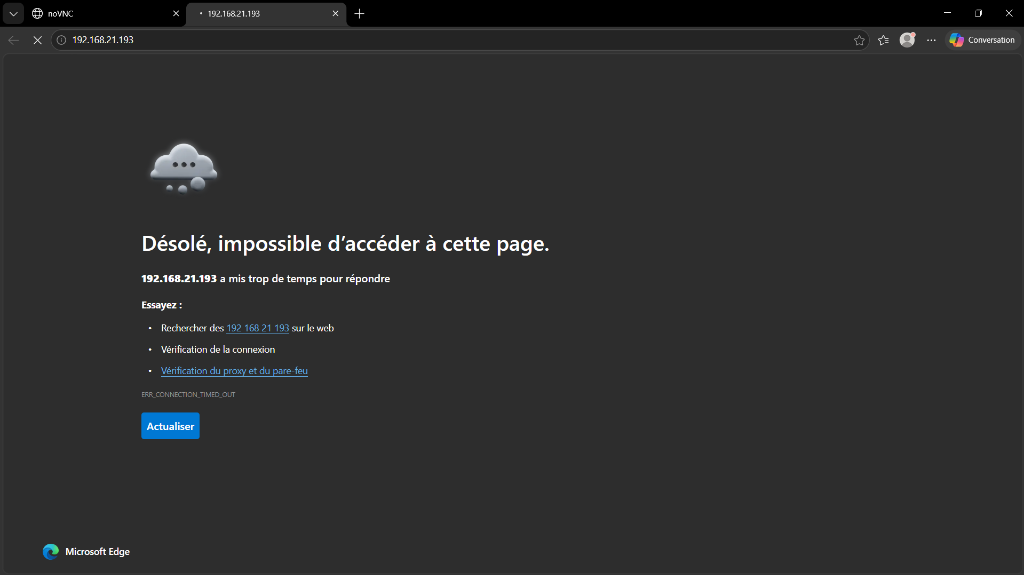
\includegraphics[width=0.8\textwidth]{screenshots/media__1775872567237.png}}
\caption{Interface de configuration r\'eseau}
\label{fig:annex_net1}
\end{figure}

\begin{figure}[H]
\centering
\fbox{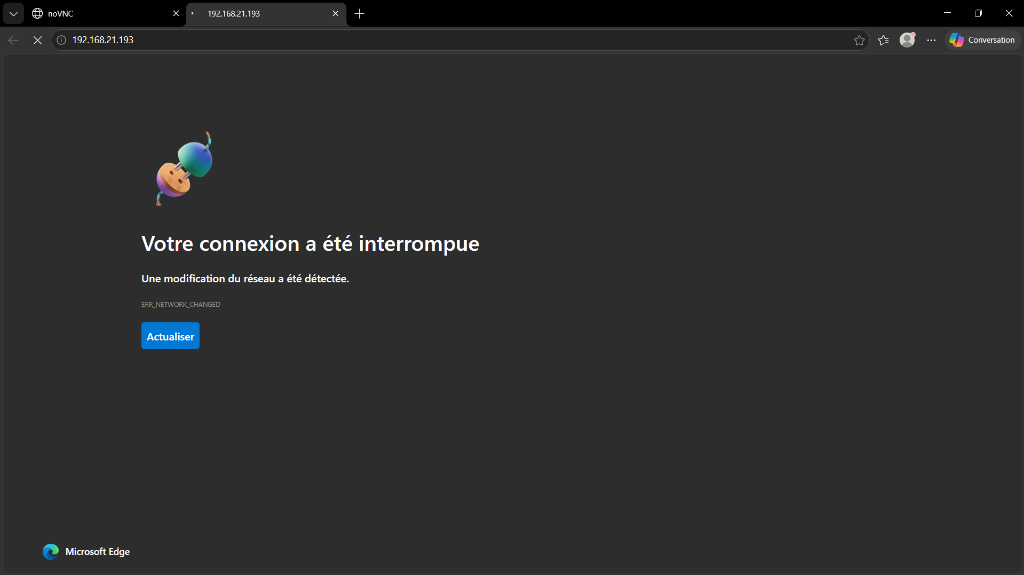
\includegraphics[width=0.8\textwidth]{screenshots/media__1775872792050.png}}
\caption{V\'erification des services OpenStack}
\label{fig:annex_services}
\end{figure}

\begin{figure}[H]
\centering
\fbox{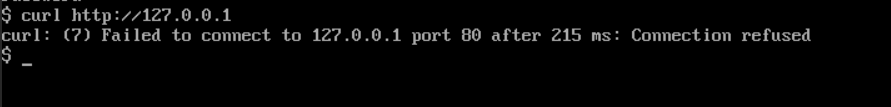
\includegraphics[width=0.8\textwidth]{screenshots/media__1775873659702.png}}
\caption{Conteneurs Docker actifs}
\label{fig:annex_docker}
\end{figure}

\begin{figure}[H]
\centering
\fbox{
\includegraphics[width=0.8\textwidth]{screenshots/media__1775874118283.png}}
\caption{Logs de d\'eploiement Kolla}
\label{fig:annex_kolla_logs}
\end{figure}

\begin{figure}[H]
\centering
\fbox{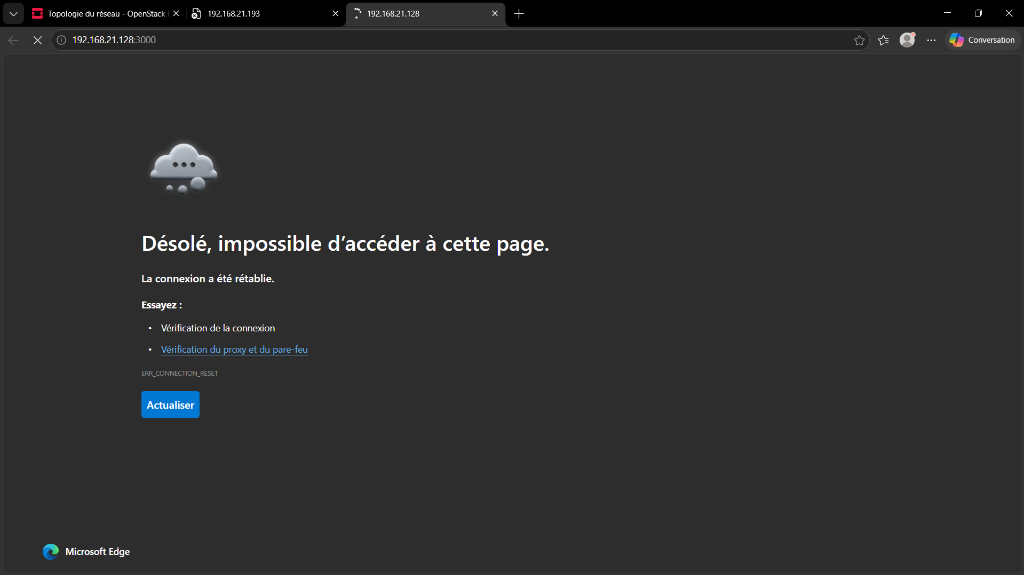
\includegraphics[width=0.8\textwidth]{screenshots/media__1775896990255.png}}
\caption{Diagnostic r\'eseau -- Ping et connectivit\'e}
\label{fig:annex_ping}
\end{figure}

\begin{figure}[H]
\centering
\fbox{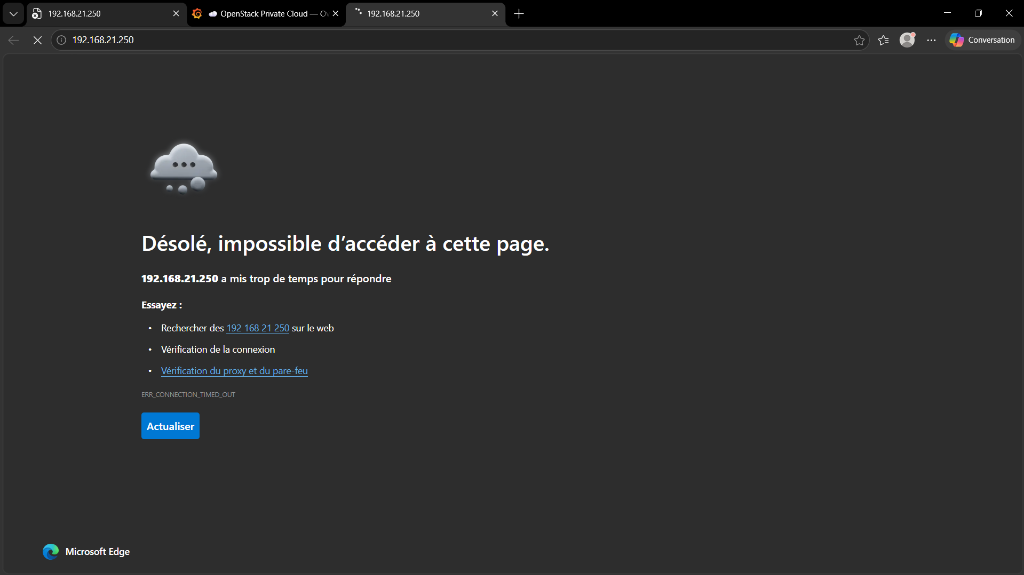
\includegraphics[width=0.8\textwidth]{screenshots/media__1775897946217.png}}
\caption{Monitoring Prometheus -- Requ\^etes PromQL}
\label{fig:annex_promql}
\end{figure}

\begin{figure}[H]
\centering
\fbox{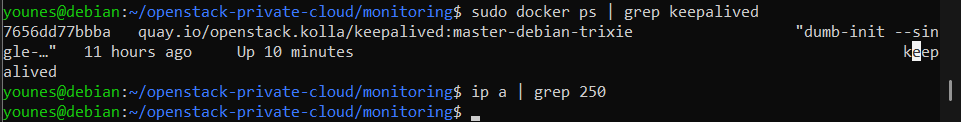
\includegraphics[width=0.8\textwidth]{screenshots/media__1775898106807.png}}
\caption{Grafana -- Configuration des sources de donn\'ees}
\label{fig:annex_grafana_ds}
\end{figure}

\begin{figure}[H]
\centering
\fbox{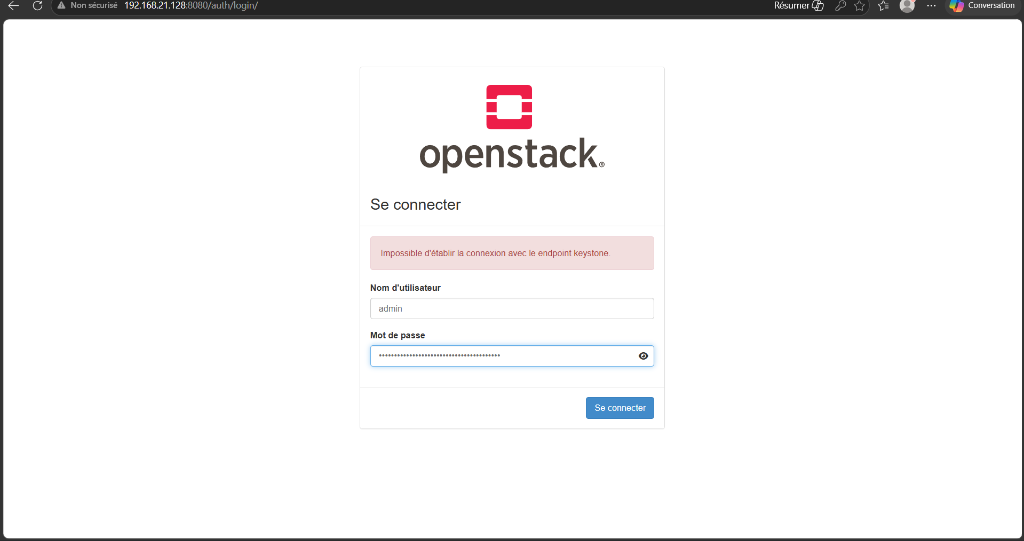
\includegraphics[width=0.8\textwidth]{screenshots/media__1775898420035.png}}
\caption{Grafana -- Dashboard CPU et m\'emoire}
\label{fig:annex_grafana_cpu}
\end{figure}

\begin{figure}[H]
\centering
\fbox{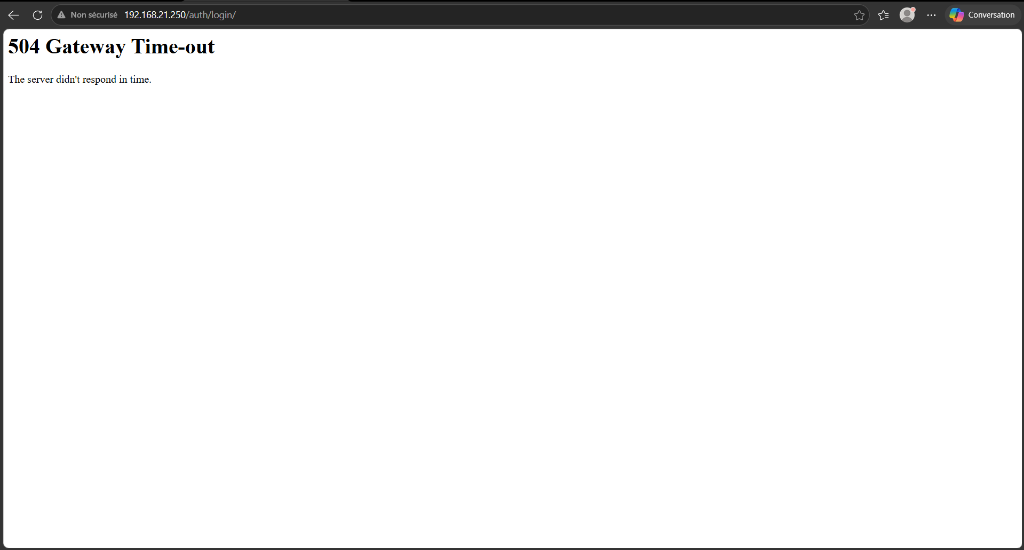
\includegraphics[width=0.8\textwidth]{screenshots/media__1775898599004.png}}
\caption{Grafana -- Statistiques de stockage}
\label{fig:annex_grafana_storage}
\end{figure}

\begin{figure}[H]
\centering
\fbox{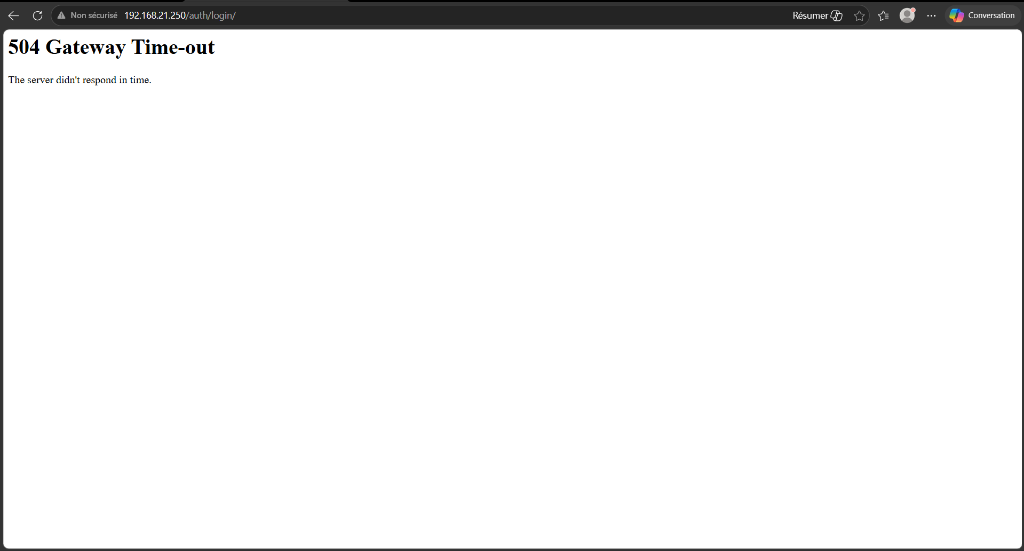
\includegraphics[width=0.8\textwidth]{screenshots/media__1775898800044.png}}
\caption{Grafana -- Vue d'ensemble conteneurs}
\label{fig:annex_grafana_containers}
\end{figure}

\begin{figure}[H]
\centering
\fbox{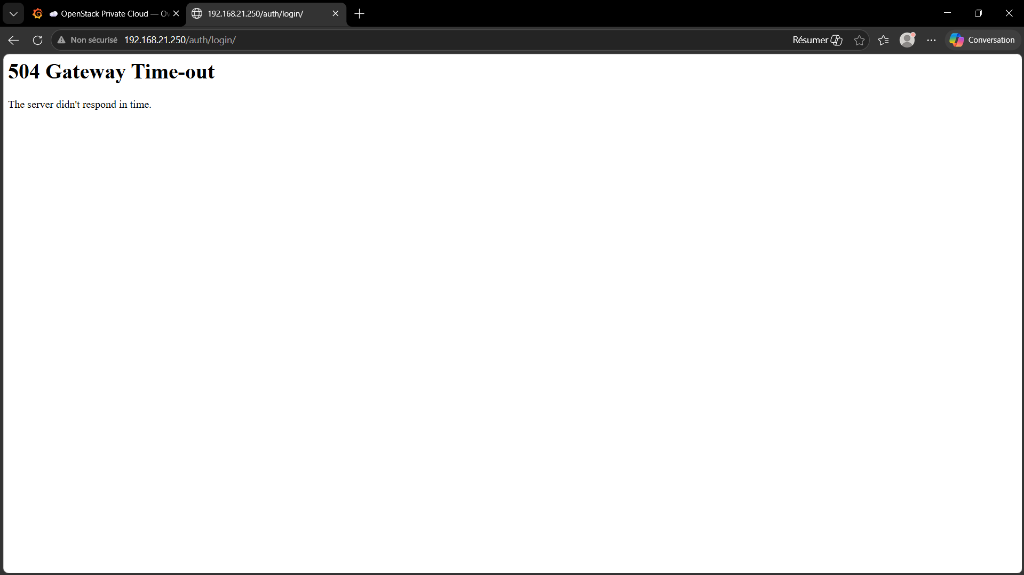
\includegraphics[width=0.8\textwidth]{screenshots/media__1775899178968.png}}
\caption{Grafana -- Alertes et r\`egles de notification}
\label{fig:annex_grafana_alerts}
\end{figure}

\begin{figure}[H]
\centering
\fbox{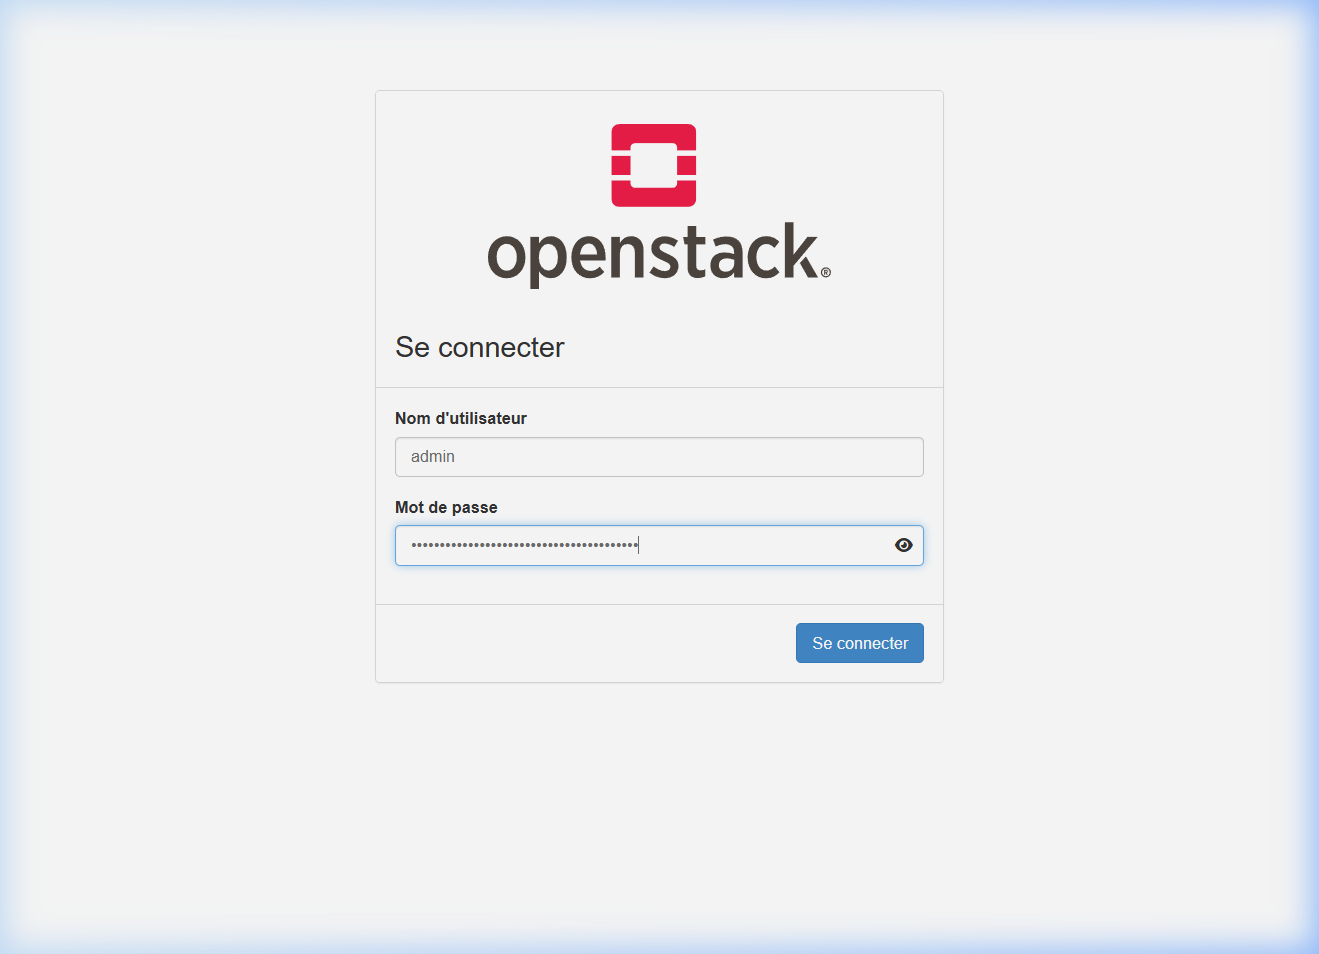
\includegraphics[width=0.8\textwidth]{screenshots/login_page_filled_1776005348321.png}}
\caption{OpenStack Horizon -- Formulaire de connexion rempli}
\label{fig:annex_login_filled}
\end{figure}


% ============================================================
% BIBLIOGRAPHIE
% ============================================================
\begin{thebibliography}{20}

\bibitem{openstack_docs} OpenStack Foundation, ``OpenStack Documentation'', \url{https://docs.openstack.org}, 2026.

\bibitem{kolla_docs} OpenStack Kolla Team, ``Kolla-Ansible Documentation'', \url{https://docs.openstack.org/kolla-ansible/latest/}, 2026.

\bibitem{terraform_docs} HashiCorp, ``Terraform Documentation'', \url{https://www.terraform.io/docs}, 2026.

\bibitem{terraform_openstack} Terraform OpenStack Provider, ``Terraform Provider for OpenStack'', \url{https://registry.terraform.io/providers/terraform-provider-openstack/openstack/latest/docs}, 2026.

\bibitem{prometheus_docs} Prometheus Authors, ``Prometheus Documentation'', \url{https://prometheus.io/docs/}, 2026.

\bibitem{grafana_docs} Grafana Labs, ``Grafana Documentation'', \url{https://grafana.com/docs/}, 2026.

\bibitem{docker_docs} Docker Inc., ``Docker Documentation'', \url{https://docs.docker.com}, 2026.

\bibitem{nist_cloud} P. Mell et T. Grance, ``The NIST Definition of Cloud Computing'', SP 800-145, NIST, 2011.

\bibitem{galera_cluster} Codership, ``Galera Cluster for MySQL/MariaDB'', \url{https://galeracluster.com/library/documentation/}, 2026.

\bibitem{keepalived_docs} Keepalived Project, ``Keepalived User Guide'', \url{https://www.keepalived.org/manpage.html}, 2026.

\bibitem{haproxy_docs} HAProxy Technologies, ``HAProxy Documentation'', \url{https://docs.haproxy.org/}, 2026.

\bibitem{ansible_docs} Red Hat, ``Ansible Documentation'', \url{https://docs.ansible.com/}, 2026.

\end{thebibliography}

\end{document}
